\documentclass{ctexart}
\usepackage{PhysicalChemistryNote}

\begin{document}\pagestyle{plain}
\setcounter{footnote}{0}
\begin{center}
    \tbf{\Huge Chapter 6 电解质溶液与电化学}
\end{center}\vspace{15pt}

\indent 电化学是物理化学中一门古老而充满活力的分支学科,它架起了化学与电学之间的桥梁,%
揭示了电能与化学能相互转化的本质规律.从伏打电池的发明到现代锂离子电池技术的革新,%
从金属腐蚀的微观机制到生物体内神经电信号的传递,电化学已深入能源,材料,环境和生命科学等众多领域.%
本章将系统探讨电化学的核心理论以及电解质溶液中离子的具体性质,%
为读者构建一个从微观离子行为到宏观电化学现象的知识框架.
\newpage\documentclass{ctexart}
\usepackage{PhysicalChemistryNote}

\begin{document}\pagestyle{plain}
\noindent\tbf{\LARGE 6A 电解质溶液}\vspace{15pt}\\
\indent 电解质溶液,例如食盐水,具有普通溶液所不具有的导电性,%
这是因为溶液中的\ce{Na^+}和\ce{Cl^-}在电场的作用下能发生定向移动,起到传递电荷的作用.%
除此之外,带异种电荷的离子之间还存在吸引力,带同种电荷的离子之间还存在排斥力.%
以上种种原因,都使得电解质溶液与一般的溶液性质并不完全相似.因此,%
我们将在本节简单的讨论其性质.\vspace{12pt}\\
\Section{6A.1 电解质溶液的电导}
\Part{电导,电导率和摩尔电导率}
\indent 物质的导电能力,通常用电阻$R$来表示.而对于电解质溶液,我们更希望直观地判断其导电能力,%
这一物理量越大,电解质溶液的导电能力就越强.因此,可以定义\tbf{电导}来衡量其导电能力.
\begin{definition}[6A.1.1 电导]
    \tbf{电导}$G$定义为电阻$R$的倒数,即$G=\dfrac1R$.
\end{definition}
导体的电阻与其长度$l$成正比,与其横截面积$S$成反比,比例系数为电阻率$\rho$,它与导体的材料有关.于是
\[R=\rho\dfrac{l}{S}\]
因此,物体的电导
\[G=\dfrac{1}{\rho}\dfrac{S}{l}\]
同样地,可以定义\tbf{电导率}以衡量材料的导电能力.
\begin{definition}[6A.1.2 电导率]
    \tbf{电导率}$\kappa$定义为电阻率$\rho$的倒数,即$\kappa=\dfrac{1}{\rho}$.
\end{definition}
对于不同浓度的溶液,其中离子的数目不同,因而导电性也是不同的.%
因此,可以定义\tbf{摩尔电导率}.
\begin{definition}[6A.1.3 摩尔电导率]
    \tbf{摩尔电导率}$\Lambda_\m$定义为溶液电阻率与摩尔浓度的之比,即$\Lambda_\m=\dfrac{\kappa}{c}$.\\
    摩尔电导率的操作定义\footnotemark 为在两个相距$1\text{ m}$的平行电极板之间充入含有$1\mol$电解质的一定浓度的溶液时具有的电导.
\end{definition}\footnotetext{操作定义,是根据可观察,可测量,可操作的特征来界定变量含义的方法.}
在讨论摩尔电导率时,需要指定电解质的基本单元.例如$\Lambda_\m(\ce{NaCl})$和$\displaystyle\Lambda_\m\left(\ce{1/2NaCl}\right)$%
在操作定义中分别指\ce{NaCl}为$1\mol$和\ce{Na^+}与\ce{Cl^-}的总量为$1\mol$.对于同一浓度的\ce{NaCl}溶液,有
\[\Lambda_\m(\ce{NaCl})=2\Lambda_\m\left(\ce{1/2NaCl}\right)\]
\Part{电导率,摩尔电导率与浓度的关系}
\indent 我们先讨论浓度与电导率的关系.几种典型的电解质溶液的电导率与浓度的关系如下图所示.
\begin{tightcenter}
    \documentclass{standalone}
\usepackage{PhysicalChemistryNote}
\begin{document}
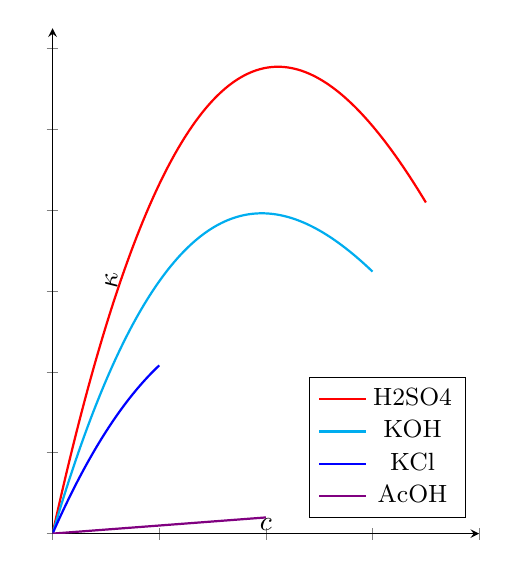
\begin{tikzpicture}
    \begin{axis}[
        width = 7cm,
        height = 8cm,
        legend pos = south east,
        xlabel = {$c$},
        ylabel = {$\kappa$},
        axis lines = left,
        x label style={at={(axis description cs:0.5,0.05)},anchor=north},
        y label style={at={(axis description cs:0.175,0.5)},rotate=0,anchor=south},
        ymax = 1.25,
        ymin = 0,
        xmax = 0.8,
        ymin = 0,
        samples = 400,
        xticklabels={},
        yticklabels={}
    ]
    \addplot [thick, red, domain=0:0.7] {3*x*(x-1)*(x-2)};
    \addlegendentry{\small{\ce{H2SO4}}}
    \addplot [thick, cyan, domain=0:0.6] {3*x*(x-1)*(x-1.5)};
    \addlegendentry{\small{\ce{KOH}}}
    \addplot [thick, blue, domain=0:0.2] {2*x*(x-1)*(x-1.5)};
    \addlegendentry{\small{\ce{KCl}}}
    \addplot [thick, violet, domain=0:0.4] {0.1*x};
    \addlegendentry{\small{\ce{AcOH}}}
    \end{axis}
\end{tikzpicture}
\end{document}
\end{tightcenter}
可以看出,在一定浓度范围内,强电解质的电导率$\kappa$随浓度的上升而上升,%
这是由于溶液中离子的浓度上升使得导电的粒子数增多;超过一定浓度范围后,$\kappa$随浓度增大而减小,%
这是由于离子变得密集,正负离子间的吸引力增大,限制了离子的导电能力所致.\\
\indent 对于弱电解质而言,$\kappa$随浓度变化不显著.浓度增大,虽然单位体积溶液的电解质分子数增多,%
但电离度却随之减小,因此离子的浓度变化不大.\\
\indent 与电导率所不同,电解质的摩尔电导率$\Lambda_\m$却总是随着浓度的增加而减小.%
几种典型的电解质溶液的电导率与浓度的关系如下图所示.
\begin{tightcenter}
    \documentclass{standalone}
\usepackage{PhysicalChemistryNote}
\begin{document}
\begin{tikzpicture}
    \begin{axis}[
        width = 8cm,
        height = 8cm,
        legend style={at={(1.05,0.5)},anchor=west},
        xlabel = {$\sqrt{c}$},
        ylabel = {$\varLambda_\m$},
        axis lines = left,
        x label style={at={(axis description cs:0.5,0.05)},anchor=north},
        y label style={at={(axis description cs:0.175,0.5)},rotate=0,anchor=south},
        ymax = 0.5,
        ymin = 0,
        xmax = 0.6,
        ymin = 0,
        samples = 400,
        xticklabels={},
        yticklabels={}
    ]
    \addplot [thick, red, domain=0:0.6] {e^(-x-3)-e^(-3)+0.45};
    \addlegendentry{\small{\ce{HCl}}}
    \addplot [thick, cyan, domain=0:0.6] {e^(-x-1)-e^(-1)+0.45};
    \addlegendentry{\small{\ce{H2SO4}}}
    \addplot [thick, blue, domain=0:0.6] {e^(-x-2)-e^(-2)+0.2};
    \addlegendentry{\small{\ce{Na2SO4}}}
    \addplot [thick, violet, domain=0:0.6] {0.4/(1+100*x)};
    \addlegendentry{\small{\ce{AcOH}}}
    \addplot [domain=0:0.6,dashed] {-e^(-3)*x+0.45};
    \addplot [domain=0:0.6,dashed] {-e^(-1)*x+0.45};
    \addplot [domain=0:0.6,dashed] {-e^(-2)*x+0.2};
    \end{axis}
\end{tikzpicture}
\end{document}
\end{tightcenter}
对于强电解质,浓度上升时两电极间的电解质数量仍保持$1\mol$,参加导电的离子数目没有变化,%
而浓度上升,离子间引力变大,离子迁移速度略有减小,于是$\Lambda_\m$随着$\sqrt{c}$的增加而缓慢减小.\\
\indent 对弱电解质,浓度上升时虽然电极间的电解质数量不变,但电离度大大减小,
导致参加导电的离子数目大大减少,于是$\Lambda_\m$随着$\sqrt{c}$的增加而迅速减小.
\end{document}
\newpage\documentclass{ctexart}
\usepackage{PhysicalChemistryNote}

\begin{document}\pagestyle{plain}
\noindent\tbf{\LARGE 6B 可逆电池的电动势}\vspace{15pt}\\
\indent 带电粒子会在电场的作用下做定向运动.对于电子而言,它总是从电势低的地方流向电势高的地方,因而形成电流.%
我们将从简单的电学和热力学出发推导电池的电动势.\\
\indent 在此之前,我们先简要介绍电势,电动势等电学中的基本概念.
\begin{definition}[6B.0.1 电势]
    电势(electric potential,简记为ePtntl)又称电位,是描述电场中某一点之能量高低性质的物理标量.%
    电场中某处的电势等于处于电场中该位置的单位电荷所具有的电势能,单位为伏特(Volt,符号为V).
\end{definition}
\begin{definition}[6B.0.2 电压]
    电压(Voltage,符号为$U$)是两点之间的电势差,也就将单位电荷从一点移动到另一点所需要的能量.
\end{definition}
\begin{definition}[6B.0.3 电动势]
    在电路学中用电动势(electromotive force,简记为emf,符号为$\mathcal{E}$或$E$)表示电源将其它形式的能量(如化学能)转化成电能的能力.%
    在电源内部,正电荷从负极被搬运至正极,电源的电动势就定义为从单位正电荷从负极移动到正极时电源提供的能量.
\end{definition}
\begin{hint}
    如果把一个闭合的电路比喻成一个循环的水流,那么电动势就是把水从低处泵到高处的水泵,%
    电动势越高就意味着水泵越有力,而电压则是水泵出水口和进水口压力差的一个表征数值.电动势表示能力属性,电压表示状态属性.
\end{hint}
电动势和电池正负极的电压由闭合电路欧姆定律关联.
\begin{theorem}[6B.0.4 闭合电路欧姆定律]
    在闭合电路中有$E=U+Ir$,其中$I$为回路电流,$r$为电池内阻,$U$为电池两极的电压.
\end{theorem}
因此,只有在回路电流$I=0$时,电池两极的电压才与电动势相等.这也是电动势测定的依据.\vspace{12pt}\\
\Section{6B.1 可逆电池}
\indent 我们在\tbf{3E.2.2}中指出,等温等压过程中系统能做的最大非体积功$W_f$等于其Gibbs自由能的减少值$\Delta G$.%
对于电池而言,这一非体积功就是电功$W_e$,Gibbs自由能的减少值就是电池反应的Gibbs自由能$\Delta_\r G$.%
由于最大功是在可逆过程中达到的,因此为了将电功与电池反应相联系,我们需要保证电池在可逆的条件下进行工作,即电池是\tbf{可逆电池}.
\begin{definition}[6B.1.1 可逆电池]
    \tbf{可逆电池}需要满足如下条件.
    \begin{enumerate}[topsep=0pt,parsep=0pt,itemsep=0pt,partopsep=0pt,label=\tbf{\arabic*.},leftmargin=*]
        \item 在无限缓慢的充放电过程中(电流趋近于零),电极反应可正向和逆向进行,电池在近平衡态的状态下工作,且能量转换可逆.
        \item 电解质中的离子迁移过程可逆.
        \item 电极反应可以逆向进行,没有不可逆的副反应(如气体析出,腐蚀等).
    \end{enumerate}
    可逆电池的电极被称作\tbf{可逆电极}.
\end{definition}
上述第一条需要外加电压才能做到,这可以与我们在\tbf{2A.3}中讨论的准静态膨胀类比.%
如果外加电压$U_\e$总是比电池电动势$\mathcal{E}$小一个无穷小量,电池就将以无穷小的电流向外放电;%
反之,如果$U_\e$总是比$\mathcal{E}$大一个无穷小量,电池就将被无穷小的电流充电.\\
\indent 如果$U_\e$与$\mathcal{E}$的差是不可忽略的常值,那么电池就将以一定的电流进行充放电.%
由于电池总是存在内阻,因此会引起发热.%
如果是向电池充电,就要向电池额外做功;如果是电池向外放电,电池向外做的功就会减少.\\
\indent 我们在\tbf{6A.2}中所说的改进版的\ce{Zn-Cu}电池就可以视作可逆电池.\vspace{12pt}\\
\Section{6B.2 Nernst方程}
\indent 现在,我们来推导可逆电池的电动势.
\begin{derivation}
    假定反应体系的组成一定.根据\tbf{5B.1.1},反应的摩尔Gibbs自由能变$\Delta_\r G_\m=\pa{G}{\xi}{T,p}$.%
    于是在等温等压和该组成下,反应进行$\di\xi$时,系统的Gibbs自由能的变化为$\di G$,满足$\dfrac{\di G}{\di\xi}=\Delta_\r G_\m$.\\
    根据\tbf{3E.2.2},体系能做的最大非膨胀功(在此时即电功)为系统Gibbs自由能的变化$\di G$,于是
    \[\delta W_e=\di G=\Delta_\r G_\m\di\xi\]
    并且要求系统以可逆电池的方式完成此过程.\\
    假定半反应中电子的计量系数为$n$,那么就有物质的量为$n\di\xi$的电子从阳极转移到阴极.%
    由于一个电子的电荷量为$-e$,因此转移电子的总电荷量$\di Q=-ne\NA\di\xi$.%
    这一过程需要对电子做的功为
    \[\delta W_e=E\di Q=-nEe\NA\di\xi=-nFE\di\xi\]
    其中Faraday常数$F=e\NA$,即$1\mol$电子的电荷的绝对值.\\
    结合上述两式,我们就有
    \[\Delta_\r G_\m=-nFE\]
    这就联系了反应Gibbs自由能变和电池的电动势.\\
    我们再考虑\tbf{5B.1.2}中标准反应Gibbs自由能变$\Delta_\r G^\ominus$和$\Delta_\r G$的关系,即
    \[\Delta_\r G_\m=\Delta_\r G^\ominus_\m+RT\ln Q\]
    代入上式可得
    \[E=-\dfrac{\Delta_\r G_\m^\ominus}{nF}-\dfrac{RT}{nF}\ln Q\]
    将有关标准反应Gibbs自由能变$\Delta_\r G_\m^\ominus$的一项定义为\tbf{标准电池电动势}$E^\ominus$,即
    \[E^\ominus=-\dfrac{\Delta_\r G_\m^\ominus}{nF}\]
    就有
    \[E=E^\ominus-\dfrac{RT}{nF}\ln Q\]
    这就是著名的Nernst方程.
\end{derivation}
\begin{theorem}[6B.2.1 Nernst方程]
    在等温等压下,某一组成时电池的电动势满足
    \[E=E^\ominus-\dfrac{RT}{nF}\ln Q\]
    其中\tbf{标准电池电动势}$E^\ominus$定义为
    \[E^\ominus=-\dfrac{\Delta_\r G_\m^\ominus}{nF}\]
    其中$\Delta_\r G_\m^\ominus$为电池反应的标准摩尔反应Gibbs自由能变.
\end{theorem}
\end{document}
\newpage\documentclass{ctexart}
\usepackage{PhysicalChemistryNote}

\begin{document}\pagestyle{plain}
\noindent\tbf{\LARGE 6C 可逆电池的电动势}\vspace{15pt}\\
\indent 带电粒子会在电场的作用下做定向运动.对于电子而言,它总是从电势低的地方流向电势高的地方,因而形成电流.%
我们将从简单的电学和热力学出发推导电池的电动势.\\
\indent 在此之前,我们先简要介绍电势,电动势等电学中的基本概念.
\begin{definition}[6C.0.1 电势]
    电势(electric potential,简记为ePtntl)又称电位,是描述电场中某一点之能量高低性质的标量.%
    电场中某处的电势等于处于电场中该位置的单位电荷所具有的电势能,单位为伏特(Volt,符号为V).
\end{definition}
\begin{definition}[6C.0.2 电压]
    电压(Voltage,符号为$U$)是两点之间的电势差,也就是将单位电荷从一点移动到另一点所需要的能量.
\end{definition}
\begin{definition}[6C.0.3 电动势]
    在电路学中用电动势(electromotive force,简记为emf,符号为$\mathcal{E}$或$E$)表示电源将其它形式的能量(如化学能)转化成电能的能力.%
    在电源内部,正电荷从负极被搬运至正极,电源的电动势就定义为从单位正电荷从负极移动到正极时电源提供的能量.
\end{definition}
\begin{hint}
    如果把一个闭合的电路比喻成一个循环的水流,那么电动势就是把水从低处泵到高处的水泵,%
    电动势越高就意味着水泵越有力,而电压则是水泵出水口和进水口压力差的一个表征数值.电动势表示能力属性,电压表示状态属性.
\end{hint}
电动势和电池正负极的电压由闭合电路欧姆定律关联.
\begin{theorem}[6C.0.4 闭合电路欧姆定律]
    在闭合电路中有$E=U+Ir$,其中$I$为回路电流,$r$为电池内阻,$U$为电池两极的电压.
\end{theorem}
因此,只有在回路电流$I=0$时,电池两极的电压才与电动势相等.这也是电动势测定的依据.\vspace{12pt}\\
\Section{6C.1 可逆电池}
\indent 我们在\tbf{3E.2.2}中指出,等温等压过程中系统能做的最大非体积功$W_f$等于其Gibbs自由能的减少值$\Delta G$.%
对于电池而言,这一非体积功就是电功$W_e$,Gibbs自由能的减少值就是电池反应的Gibbs自由能$\Delta_\r G$.%
由于最大功是在可逆过程中达到的,因此为了将电功与电池反应相联系,我们需要保证电池在可逆的条件下进行工作,即电池是\tbf{可逆电池}.
\begin{definition}[6C.1.1 可逆电池]
    \tbf{可逆电池}需要满足如下条件.
    \begin{enumerate}[topsep=0pt,parsep=0pt,itemsep=0pt,partopsep=0pt,label=\tbf{\arabic*.},leftmargin=*]
        \item 在无限缓慢的充放电过程中(电流趋近于零),电极反应可正向和逆向进行,电池在近平衡态的状态下工作,且能量转换可逆.
        \item 电解质中的离子迁移过程可逆.
        \item 电极反应可以逆向进行,没有不可逆的副反应(如气体析出,腐蚀等).
    \end{enumerate}
    可逆电池的电极被称作\tbf{可逆电极}.
\end{definition}
上述第一条需要外加电压才能做到,这可以与我们在\tbf{2A.3}中讨论的准静态膨胀类比.%
如果外加电压$U_\e$总是比电池电动势$\mathcal{E}$小一个无穷小量,电池就将以无穷小的电流向外放电;%
反之,如果$U_\e$总是比$\mathcal{E}$大一个无穷小量,电池就将被无穷小的电流充电.\\
\indent 如果$U_\e$与$\mathcal{E}$的差是不可忽略的常值,那么电池就将以一定的电流进行充放电.%
由于电池总是存在内阻,因此会引起发热.%
如果是向电池充电,就要向电池额外做功;如果是电池向外放电,电池向外做的功就会减少.\\
\indent 因此,以可逆的方式向电池充电消耗的电能最少,而电池以可逆的方式放电放出的电能最多.%
这和我们在讨论可逆膨胀/压缩时得出的结论是类似的,只是能量转化的形式不同.\\
\indent 我们在\tbf{6A.2}中所说的改进版的\ce{Zn-Cu}电池就可以视作可逆电池.\vspace{12pt}\\
\Section{6C.2 Nernst方程}
\Part{Nernst方程}
\indent 现在,我们来推导可逆电池的电动势.
\begin{derivation}
    假定反应体系的组成一定.根据\tbf{5B.1.1},反应的摩尔Gibbs自由能变$\Delta_\r G_\m=\pa{G}{\xi}{T,p}$.%
    于是在等温等压和该组成下,反应进行$\di\xi$时,系统的Gibbs自由能的变化为$\di G$,满足$\dfrac{\di G}{\di\xi}=\Delta_\r G_\m$.\\
    根据\tbf{3E.2.2},体系能做的最大非膨胀功(在此时即电功)为系统Gibbs自由能的变化$\di G$,于是
    \[\delta W_e=\di G=\Delta_\r G_\m\di\xi\]
    并且要求电池以可逆的方式完成此过程.\\
    假定半反应中电子的计量系数为$\nu$,那么就有物质的量为$\nu\di\xi$的电子从阳极转移到阴极.%
    由于一个电子的电荷量为$-e$,因此转移电子的总电荷量$\di Q=-\nu\e\NA\di\xi$.%
    这一过程需要对电子做的功为
    \[\delta W_e=E\di Q=-\nu Ee\NA\di\xi=-\nu FE\di\xi\]
    其中Faraday常数$F=e\NA$,即$1\mol$电子的电荷量的绝对值.\\
    结合上述两式,我们就有
    \[\Delta_\r G_\m=-\nu FE\]
    这就联系了反应Gibbs自由能变和电池的电动势.\\
    我们再考虑\tbf{5B.1.2}中标准反应Gibbs自由能变$\Delta_\r G^\ominus$和$\Delta_\r G$的关系,即
    \[\Delta_\r G_\m=\Delta_\r G^\ominus_\m+RT\ln Q\]
    代入上式可得
    \[E=-\dfrac{\Delta_\r G_\m^\ominus}{\nu F}-\dfrac{RT}{\nu F}\ln Q\]
    将有关标准反应Gibbs自由能变$\Delta_\r G_\m^\ominus$的一项定义为\tbf{标准电池电动势}$E^\ominus$,即
    \[E^\ominus=-\dfrac{\Delta_\r G_\m^\ominus}{\nu F}\]
    就有
    \[E=E^\ominus-\dfrac{RT}{\nu F}\ln Q\]
    这就是著名的Nernst方程.
\end{derivation}
\begin{theorem}[6C.2.1 Nernst方程]
    在等温等压下,某一组成时电池的电动势满足
    \[E=E^\ominus-\dfrac{RT}{\nu F}\ln Q\]
    其中\tbf{标准电池电动势}$E^\ominus$定义为
    \[E^\ominus=-\dfrac{\Delta_\r G_\m^\ominus}{\nu F}=\dfrac{RT\ln K^\ominus}{\nu F}\]
    其中$\nu$为反应转移的电子的计量数,$\Delta_\r G_\m^\ominus$为电池反应的标准摩尔反应Gibbs自由能变,$K^\ominus$为反应的标准平衡常数.
\end{theorem}
Nernst方程揭示了电池电动势与反应商$Q$之间的关联.需要注意的是,尽管反应物和产物可能被盐桥等导电物质隔离,%
反应商依然是存在的,并不要求它们混合.%
回忆我们在\tbf{5B.1.4}中的推导,是从化学势推出反应商$Q$这一概念,%
而溶质的化学势与其它溶质存在与否并无关联,只与溶质本身的浓度相关.%
这也启示我们可以把阴极和阳极分开考虑,我们将在\tbf{6D}中详细讨论这一点.\vspace{4pt}\\
\Part{热力学函数的测定}
\indent 根据Nernst方程可以将$E$与$\Delta_\r G_\m$联系起来,而电动势的测定是可以做到比较精准的%
(至少比一般的量热计要精确得多),因此测量$E$也可以间接地推定反应的热力学数据.
\begin{derivation}
    我们知道$\pa GTp=-S$,因此
    \[\pa{\Delta_\r G_\m}Tp=-\Delta_\r S_\m\]
    将Nernst方程$\Delta_\r G_\m=-\nu EF$代入可得
    \[\Delta_\r S_\m=\nu F\pa ETp\]
    又因为$\Delta_\r H_\m=\Delta_\r G_\m+T\Delta_\r S_\m$,于是
    \[\Delta_\r H_\m=-\nu FE+\nu FT\pa ETp\]
    保持压强一定,测定$E$随温度$T$的变化关系,就可以求出对应温度下的$\Delta_\r H_\m$与$\Delta_\r S_\m$.%
    需要注意的是此时测得的数据是对应于特定组成的电池的,并不是反应的标准焓变或熵变.
\end{derivation}
\Section{6C.3 电池电动势的产生原理}
\indent 一个电池总的电动势的产生是比较复杂的.我们现在来分别介绍几种主要的电动势及其产生原因.\vspace{4pt}\\
\Part{电极与电解质溶液界面电势}
\indent 金属晶格中有金属离子和能够自由移动的电子存在\footnote{你应当在结构化学中学习过这一点.}.%
当我们把金属单质\ce{M}浸入含对应金属离子\ce{M^n+}的溶液时,如果\ce{M^n+}在金属中和在溶液中的化学势不相等,%
就会发生转移.根据溶液中\ce{M^n+}浓度的不同,这可能发生两种情形:\ce{M^n+}从单质转移至溶液,电子留在单质中;%
使得金属带负电,溶液带正电;%
或是\ce{M^n+}从溶液转移至单质,使得溶液带负电,金属带正电.\\
\indent 无论何种情形,都会导致两相带上相反的电荷,从而使得界面出现电势差.%
同时,由于静电作用,这一电势差会阻止金属离子继续发生转移,从而很快地达成平衡,于是两相的电势差也趋于稳定.\\
\indent 在静电作用下,金属相所带的电荷是集中在表面的,而溶液中的带异号电荷的离子一方面受到金属表面电荷的吸引,趋向于紧靠金属表面;%
另一方面,离子的热运动使得它们又会趋向于平均地分布在溶液中.%
当静电吸引与热运动分散平衡时,在电极与溶液界面处就形成了一个\tbf{双电层}\footnote{双电层最早由Helmholtz提出并模型化,在不断优化下形成Gouy-Chapman-Stern模型.%
关于双电层理论的演化历史,可以参考https://zhuanlan.zhihu.com/p/27155545.}.
\begin{definition}[6C.3.1 双电层]
    \tbf{双电层}是由电极表面上的电荷层与溶液中过剩的反号离子层构成,这一离子层又分为\tbf{紧密层}和\tbf{扩散层}两部分.%
    与金属靠的较为紧密的一层称为紧密层,除此之外扩散到溶液中去的称为扩散层.
\end{definition}
一般而言,紧密层的厚度约为$0.1\text{ nm}$,而扩散层的厚度与溶液的浓度,金属的电荷以及温度等有关.%
溶液浓度越大,分散层厚度越小,其厚度通常在$10^{-10}\sim10^{-6}\text{m}$之间.\\
\indent 如果规定溶液本体中的电位为$0$,电极相的电位为$\ep$,则电极与溶液界面电势差就是$\ep$.$\ep$在双电层中的分布情况如下图所示,%
是紧密层电位$\psi_1$和扩散层电位$\psi_2$的加和值.
\begin{tightcenter}
    \documentclass{standalone}
\usepackage{PhysicalChemistryNote}
\begin{document}
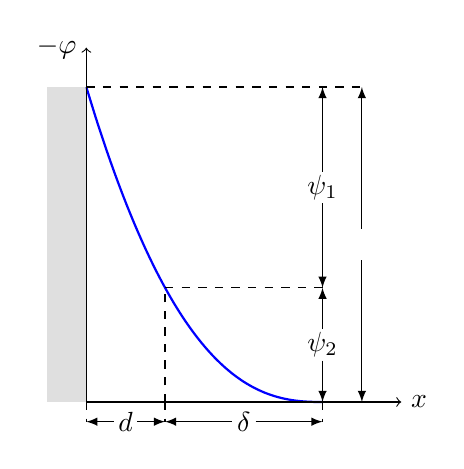
\begin{tikzpicture}
    \draw[domain=0:3,thick,blue] plot[smooth](\x,{(3-\x)^(2.5)/(3^2.5)*4});
    \draw[->] (0,0)--(4,0) node[right]{$x$};
    \draw[->] (0,0)--(0,4.5) node[left]{$-\varphi$};
    \draw[dashed] (1,0)--(1,{(2^2.5)/(3^2.5)*4});
    \draw[dashed] (0,4)--(3.5,4);
    \draw[dashed] (1,{(2^2.5)/(3^2.5)*4})--(3,{(2^2.5)/(3^2.5)*4});
    \draw[dashed] (1,0)--(1,-0.25);
    \draw[dashed] (3,0)--(3,-0.25);
    \draw[dashed] (0,0)--(0,-0.25);
    \node at (3,{(2^2.5)/(3^2.5)*2}) {$\psi_2$};
    \node at (3,{(2^2.5)/(3^2.5)*2+2}) {$\psi_1$};
    \node at (3.5,2) {$\ep$};
    \node at (0.5,-0.25) {$d$};
    \node at (2,-0.25) {$\delta$};
    \draw[-latex] (3,{(2^2.5)/(3^2.5)*2-0.2})--(3,0);
    \draw[-latex] (3,{(2^2.5)/(3^2.5)*2+0.2})--(3,{(2^2.5)/(3^2.5)*4});
    \draw[-latex] (3,{(2^2.5)/(3^2.5)*2+1.8})--(3,{(2^2.5)/(3^2.5)*4});
    \draw[-latex] (3,{(2^2.5)/(3^2.5)*2+2.2})--(3,4);
    \draw[-latex] (3.5,1.8)--(3.5,0);
    \draw[-latex] (3.5,2.2)--(3.5,4);
    \draw[-latex] (2.15,-0.25)--(3,-0.25);
    \draw[-latex] (1.85,-0.25)--(1,-0.25);
    \draw[-latex] (0.65,-0.25)--(1,-0.25);
    \draw[-latex] (0.35,-0.25)--(0,-0.25);
    \fill[lightgray,opacity=0.5] (-0.5,0)rectangle(0,4);
\end{tikzpicture}
\end{document}
\end{tightcenter}
图中的灰色区域表示金属,横坐标$x$为距离金属表面的距离,纵坐标$-\varphi$为对应位置的负电势.\\
\indent 事实上,我们将在\tbf{6C.3}中讨论的电极电势指的就是电极与电解质溶液的界面电势.%
关于这一点,之后会给出更详细的解释.\vspace{4pt}\\
\Part{接触电势}
\indent 对于不同的金属,其电子具有的能量也不同,Fermi能级\footnote{音译为费米.$0\K$下Fermi能级定义为电子能占据的最高能级,在一般温度下Fermi能级定义为电子有50\%概率占据的能级.%
简单来说,Fermi能级衡量了一个系统中电子的平均能量,当两个系统接触时电子将从Fermi能级高的系统移动至Fermi能级低的系统,直至两个系统的Fermi能级相同.这一概念与系统的化学势有十分密切的关联.\\
\indent 关于Fermi能级的形象概念,你也可以参考https://www.zhihu.com/question/22560362/answer/2180449510.}也不同.%
当这两种不同的金属接触时,电子会从Fermi能级高的金属流入Fermi能级低的金属,直至达到平衡.%
这一过程会使得两种金属带上相反的电荷,从而使得界面出现电势差.这就是\tbf{接触电势}.
\begin{definition}[6C.3.2 接触电势]
    \tbf{接触电势}是由于两个或多个材料接触面上存在不同程度的电子互相转移和表面电荷分布不均所产生的电势差.
\end{definition}
由于我们一般要用导线将两个电极相连,而导线又以铜质导线居多,因此接触电势在大部分情况下都是存在的.\vspace{4pt}\\
\Part{液体接界电势}
\indent 液体接界电势,即我们在\tbf{6A.2}所说的\tbf{液接电势},是由于两个组成不同的溶液之间存在离子扩散速率的差异导致的.%
例如在两种浓度不同的\ce{HCl}溶液的界面上,由于\ce{H^+}的扩散速率明显快于\ce{Cl^-},%
因此越过界面的\ce{H^+}就比\ce{Cl^-}多,使较稀的一侧出现过量\ce{H^+},%
较浓的一侧剩余过量\ce{Cl^-},从而使得界面出现电势差.%
这一电势差反过来会加速\ce{Cl^-}的扩散,减缓\ce{H^+}的扩散,%
最终两种离子扩散速率相等时的电势差即为\tbf{液接电势}.
\begin{definition}[6C.3.2 液体接界电势]
    \tbf{液体接界电势}是由于组成不同的溶液界面上各种离子扩散速率不同所产生的电势差.
\end{definition}
为了减小液体接界电势的影响,我们通常在两个溶液之间用盐桥连接,使液接电位降低或接近于消除.%
以饱和\ce{KCl}盐桥为例,由于其浓度很高,因此盐桥与两边溶液各自的界面上主要发生\ce{K^+}和\ce{Cl^-}的扩散.%
由于\ce{K^+}和\ce{Cl^-}的扩散速率几乎相等,所以在两个界面上只会产生两个数值很小且几乎相等,方向相反的液接电位,%
从而在很大程度上减小液接电势.\vspace{4pt}\\
\Part{电池电动势的组成}
\indent 上述几种电势共同组成了电池的电动势.以\ce{Zn-Cu}电池为例,其电池电动势的来源为
\vspace{-5pt}\begin{table}[H]\centering
    \begin{tabular}{ccccccccc}
        \ce{Cu(s)} &$\vert$ &\ce{Zn(s)}   &$\vert$ &\ce{ZnSO4(aq)} &$\vert$    &\ce{CuSO4(aq)} &$\vert$    &\ce{Cu(s)}\\
                &$\varphi_{\text{接触}}$    &&$\ep_{-}$&&$\varphi_{\text{液接}}$&&$\ep_{+}$
    \end{tabular}
\end{table}\vspace{-15pt}
为了表示接触电势,将与\ce{Zn}相连的\ce{Cu}写在最左边.这样,电池的电动势$E$就满足
\[E=\varphi_{\text{接触}}+\varphi_{\text{液接}}+\ep_-+\ep_+\]
虽然$\ep_-$和$\ep_+$的值难以测量,但我们在\tbf{6D}中将介绍电极电势,以此将$\ep$转化为一个可测的常量.\vspace{12pt}\\
\Section{6C.4 电动势的测定\footnote{本节内容仅需了解即可,不必掌握.}}
\Part{Poggendorff对消法测电动势}
\indent 可逆电池的电动势不能直接用电压表来测定.使用电压表读数时,回路中有一定的电流,%
这使得此时的电池并不是可逆电池,并且测得的也只是电池的正负极电压而非其电动势.%
因此,测定可逆电池的电动势需要在几乎没有电流通过的情况下进行.
\begin{center}
    \documentclass{standalone}
\usepackage{PhysicalChemistryNote}
\begin{document}
\begin{tikzpicture}
    \draw[-] (0,0)--(1,0);
    \draw[-] (1.9,-1)--(1,-1)--(1,1)--(1.9,1);
    \draw[-] (2.1,-1)--(3,-1)--(3,-0.25);
    \draw[-] (3,0.25)--(3,1)--(2.1,1);
    \draw[-] (3,0.25)--(3.5,0)--(4.7,0);
    \draw[-] (5.3,0)--(6.5,0);
    \draw[-latex] (6.5,0)--(6.5,2.85);
    \draw[-] (0,0)--(0,3)--(2,3);
    \draw[-] (9,3)--(10,3)--(10,4);
    \draw[-] (0,3)--(0,4)--(2.9,4);
    \draw[-] (3.1,4)--(6.5,4);
    \draw[-] (7.5,4)--(10,4);
    
    \draw[thick] (5,0) circle (0.3);
    \draw[draw=black,fill=white] (3.5,0) circle (0.05);
    \draw[draw=black,fill=white] (3,-0.25) circle (0.05);
    \draw[draw=black,fill=white] (3,0.25) circle (0.05);
    \draw[draw=black,fill=white,thick] (2,2.85)rectangle(9,3.15);
    \draw[draw=black,fill=white,thick] (6.5,3.85)rectangle(7.5,4.15);
    \draw[-latex] (6.6,3.6)--(7.4,4.4);

    \draw[-,thick] (1.9,0.85)--(1.9,1.15);
    \draw[-,thick] (2.1,0.75)--(2.1,1.25);
    \draw[-,thick] (1.9,-0.85)--(1.9,-1.15);
    \draw[-,thick] (2.1,-0.75)--(2.1,-1.25);
    \draw[-,thick] (2.9,3.85)--(2.9,4.15);
    \draw[-,thick] (3.1,3.75)--(3.1,4.25);

    \node at (2,1.5) {$E_x$};
    \node at (2,-1.5) {$E_{\text{s.c.}}$};
    \node at (3,4.5) {$E_{w}$};
    \node at (7,4.5) {$R$};
    \node[below right] at (3.5,0) {$K$};
    \node at (5,0) {$G$};
    \node[below] at (2,2.85) {$A$};
    \node[below] at (9,2.85) {$B$};

\end{tikzpicture}
\end{document}
\end{center}
Poggendorff对消法就是依据上述条件设计的测定电源电动势的方法,其电路图如上所示.%
我们现在来介绍其具体步骤.
\begin{solution}
    工作电源$E_w$在均匀的电阻丝$AB$上产生均匀的压降(这可以由欧姆定律得出).\\
    首先将开关$K$打到上端,使得待测电源$E_x$接入电路.调节$AB$上的滑动点,使得灵敏电流计$G$的示数为$0$.%
    记此时滑动点的位置为$X$,则由于电流$I=0$而$E_x$的电动势与$AX$上的电压相等.\\
    现在将开关$K$打到下端,使得标准电源$E_{\text{s.c.}}$接入电路.同样调节滑动电使$G$的实数为$0$,%
    记此时滑动点的位置为$P$.这样,$E_{\text{s.c.}}$的电动势与$AP$上的电压相等.\\
    考虑上半部分电路的欧姆定律,有
    \[E_x=U_{AX}=I_wR_{AX}=I_w\rho\dfrac{\overline{AX}}{S}\]
    \[E_{\text{s.c.}}=U_{AP}=I_wR_{AP}=I_w\rho\dfrac{\overline{AP}}{S}\]
    其中$\rho$为电阻丝的电阻率,$S$为其横截面积.这样就有
    \[E_x=\dfrac{\overline{AX}}{\overline{AP}}E_{\text{s.c.}}\]
    测定相关的长度,就可以由标准电池的电动势得到待测电池的电动势.
\end{solution}
\Part{Weston标准电池}
\indent 我们在Poggendorff对消法中需要一个电势已知的标准电池.常用的标准电池是\tbf{Weston标准电池},%
可以表示如下.
\[\ce{Cd(Hg)}\vert\ce{CdSO4.8/3H2O(s)}\vert\ce{CdSO4(aq)}\vert\ce{CdSO4.8/3H2O(s)}\vert\ce{Hg,Hg2SO4}\vert\ce{Hg}\]
电池的负极为镉汞齐,正极是\ce{Hg}与\ce{Hg2SO4}的混合糊状物.为了正极与导线更好接触,在正极下再置入一层\ce{Hg}单质.%
正极和负极表面均覆盖有$\displaystyle\ce{CdSO4.8/3H2O(s)}$,然后用\ce{CdSO4}饱和溶液连接两极.\\
\indent 电池的电动势是稳定的,并且只与镉汞齐中\ce{Cd}的活度有关,%
而\ce{Cd}的活度在一定温度下是定值.因此,Weston标准电池的电动势只与温度$T$有关.%
根据温度查阅相关数据即可得出其电动势.
\end{document}
\newpage\documentclass{ctexart}
\usepackage{PhysicalChemistryNote}

\begin{document}\pagestyle{plain}
\noindent\tbf{\LARGE 6D 电化学势与电极电势}\vspace{15pt}\\
\indent 氧化还原反应中的半反应和电池的电极让我们可以单独地对一个氧化还原电对进行研究.%
正如物质有其氧化性强弱之分,电极的电势也有高低之分.在研究电极的电势之前,%
我们需要引入电化学势这一概念对电极作更深刻的了解.\vspace{12pt}\\
\Section{6D.1 电化学势}
\Part{电化学势}
\indent 一直以来,我们研究的系统中所有组分均为电中性的.而在电池中,大部分粒子都是带电粒子,%
这意味着它们的转移与变化不仅与它在某一处化学势$\mu$有关,也与该处的电势$\phi$有关.%
因此,我们需要综合考虑上述两种情形,并由此定义\tbf{电化学势}.
\begin{definition}[6D.1.1 电化学势]
    带电粒子$i$在$\alpha$处的\tbf{电化学势}$\overline{\mu}_i^\alpha$,定义为$i$在此处的摩尔电势能与化学势之和,即
    \[\overline{\mu}_i^\alpha=\mu_i^\alpha+z_iF\phi^\alpha\]
    其中$\mu_i^\alpha$为$i$在$\alpha$处的化学势,$z_i$为$i$的电荷数,$F$为Faraday常数,$\phi^\alpha$为$\alpha$处的电势.
\end{definition}
我们现在来说明这一定义(即简单相加)的合理性.
\begin{derivation}
    我们考虑将物质的量为$\di n_i$的带电粒子$i$从系统的$\alpha$处移动到系统的$\beta$处.%
    系统的Gibbs自由能变化为
    \[\di G=\di G^\alpha+\di G^\beta=-\mu_i^\alpha\di n_i+\mu_i^\beta\di n_i=\left(\mu_i^\beta-\mu_i^\alpha\right)\di n_i\]
    这一过程做的电功(注意功的符号,正电荷从电势低处移向电势高处时系统做负功)为
    \[\delta W_e=-\Delta\phi\di Q=\left(\phi^\alpha-\phi^\beta\right)z_ie\NA\di n_i=\left(\phi^\alpha-\phi^\beta\right)z_iF\di n_i\]
    根据\tbf{3E.2.2},如果$\di G<\delta W_e$,那么这一转移就是自发的,即
    \[\mu_i^\beta+z_iF\phi^\beta<\mu_i^\alpha+z_iF\phi^\alpha\]
    因此,我们把$\mu_i^\alpha+z_iF\phi^\alpha$定义为$i$在$\alpha$处的电化学势,%
    并由此可得等温等压下带电粒子$i$总是向电化学势小的地方迁移.因此,在研究含有带电粒子的系统时,%
    我们可以用电化学势代替原来的化学势对系统的热力学性质进行研究.
\end{derivation}
由此,我们可以得出与\tbf{4B.3.4}相似的结论.
\begin{definition}[6D.1.2 含带电粒子的多组分体系自发变化的方向]
    等温等压下的多组分封闭体系中,任意组分总是从电化学势大的地方转移至电化学势小的地方,%
    直到该组分在系统各处的电化学势相等.
\end{definition}
我们现在再次考虑两种金属接触时产生接触电势的现象.尽管我们已经知道,%
两种金属的界面两侧确实存在电势差,但电压表测得的数据却是$0$.对于这一点,我们给出以下结论.
\begin{theorem}[6D.1.3 电压的实际测定值]
    电压表(包括其它用电路方法测定电压的手段)实际上测定的是两点之间电子的电化学势之差,%
    两者之间成正比例关系,比例系数为Faraday常数$F$.
\end{theorem}
\begin{proof}
    如果我们希望用电压表测定$a,b$两点之间的“电压”,就会把电压表接在$a,b$两点之间.%
    由于我们使用的是导线,因此电压表实际上接受的是两端导线内的电势差.\\
    在导线分别与两点的界面上,电子的电化学势相等,即
    \[\overline{\mu}_\e^a=\overline{\mu}_\e^{a'}\ \ \ \ \ 
    \overline{\mu}_\e^b=\overline{\mu}_\e^{b'}\]
    其中$\overline{\mu}_\e^{a'}$为电压表所连导线的电子的电化学势,$\overline{\mu}_\e^{b'}$同理.根据电化学势的定义有
    \[\overline{\mu}_\e^{a'}=\mu^{a'}_\e-F\phi^a\ \ \ \ \ 
    \overline{\mu}_\e^{b'}=\mu^{b'}_\e-F\phi^b\]
    而导线的材料相同,即$\mu^{a'}_\e=\mu^{b'}_\e$,因此
    \[\phi^b-\phi^a
    =\dfrac{\left(\mu^{b'}_\e-\overline{\mu}_\e^{b'}\right)-\left(\mu^{a'}_\e-\overline{\mu}_\e^{a'}\right)}{F}
    =\dfrac{\overline{\mu}_\e^{a'}-\overline{\mu}_\e^{b'}}{F}
    =\dfrac{\overline{\mu}_\e^a-\overline{\mu}_\e^b}{F}\]
    由此,我们可以知道尽管电压表理论上测定的是两点的电压,%
    但由于材料不同而造成的接界电势存在,电压表实际上测定的是两点电子的电化学势之差.\\
    由于相同的原因,其它使用电路学原理测定电压的方法事实上都是测定电子的电化学势之差.%
    只不过在物理的范畴中,通常不考虑电子在不同材料中的化学势之差.%
    此时,电化学势差与电势差成正比例关系,因此我们说电压表测定的是两点的电压.
\end{proof}
我们以\ce{Ti}和\ce{Au}接触为例.电子在两种金属中的化学势,%
可以由其逸出功\footnote{源于Albert Einstein对光电效应的解释,即电子从固体内部移到固体外部所必需的最小能量.%
固体的逸出功与其Fermi能级密切相关.}定性判断.%
\ce{Ti}的逸出功为$4.33\text{ eV}$,而\ce{Au}的逸出功为$5.10\text{ eV}$.%
由于\ce{Au}中的电子更难被移出,因此电子在\ce{Au}中的化学势更低.%
当两者接触时,电子发生转移,直至各处的$\overline{\mu}_\e$相同.%
此时尽管$\phi^{\ce{Ti}}<\phi^{\ce{Au}}$,电压表却无法给出这一电势的具体值,%
而只能给出电子的电化学势之差.\\
\indent 由此,我们可以更明确地定义电极电势的概念.\vspace{12pt}\\
\Section{6D.2 电极电势}
\Part{电极电势}
\indent 正如\tbf{6D.1.3}所述,只要知道电极的电化学势,%
就可以知道它们组合形成的电池的电动势,进而与我们在\tbf{6C}的内容联系起来.\\
\indent 然而,化学势和电势的绝对值都是无法得知的,这意味着电化学势亦不能被直接量度,%
只能通过具体电池的电动势间接地推定.如果确定一个\tbf{标准电极},%
就能由电极与这一标准电极所组成电池的电动势衡量其电极的电化学势,即\tbf{电极电势}.
\begin{definition}[6D.2.1 电极电势]
    电极的\tbf{电极电势}即与标准电极组成电池的电动势.%
    以标准电极为阳极,该电极的电极电势与组成电池电动势符号一致.
\end{definition}
按照IUPAC于1953年的建议,采用\tbf{标准氢电极(SHE)}作为标准电极,这一建议得到了广泛地承认和应用.%
SHE的由镀铂黑的铂完全浸入活度$a=1$的\ce{H^+}溶液,然后不断向其表面鼓入分压为$p^\ominus$的\ce{H2}所制成的电极%
\footnote{选择铂黑是因为\ce{H2}不导电,需要用合适的金属将其吸附后再建立\ce{2H^+ + 2e^- <=> H2}的平衡,%
而最佳的材料为镀有铂黑的铂.}.\\
\indent 以\ce{Cu^2+/Cu}电极为例,电极由\ce{Cu}单质浸入活度$a=1$的\ce{Cu^2+}溶液,其电极电势
\[\varphi_{\ce{Cu^2+/Cu}}=0.334\text{ V}\]
即用此电极与SHE构成的电池的电动势为$0.334\text{ V}$.%
对于任意两个电极形成的电池,其电动势即两个电极的电极电势之差.%
我们将在\tbf{6D.3}中证明这一点.\vspace{4pt}\\
\Part{电极反应的Nernst方程}
\indent 既然电动势能被写作两个电极的电极电势之差,那么电动势的Nernst方程也应当对应电极电势的Nernst方程.
\begin{derivation}
    考虑氧化还原电极,假定电极半反应为\ce{Ox(aq) + $\nu$e^- <=> Red(aq)}.假定此电极作为阴极,%
    根据Nernst方程,它与SHE形成的电池电动势满足
    \[E=E^\ominus+\dfrac{RT}{\nu F}\ln\dfrac{a_{\ce{Ox}}a_{\ce{H2}}^{\frac\nu2}}{a_{\ce{Red}}a_{\ce{H^+}}^\nu}
    =E^\ominus+\dfrac{RT}{\nu F}\ln\dfrac{a_{\ce{Ox}}}{a_{\ce{Red}}}\]
    这是因为SHE中\ce{H2}和\ce{H^+}的活度均为$1$.由于上述$E$和$E^\ominus$均是相对SHE的电动势,因此就是电极电势.我们把上式改写为
    \[\varphi_{\ce{Ox/Red}}=\varphi^\ominus_{\ce{Ox/Red}}+\dfrac{RT}{\nu F}\ln\dfrac{a_{\ce{Ox}}}{a_{\ce{Red}}}\]
    这就是电极反应的Nernst方程.
\end{derivation}
\begin{theorem}[6D.2.2 电极反应的Nernst方程]
    对于氧化还原对\ce{Ox/Red}构成的电极,若其半反应为\ce{Ox + $\nu$e^- <=> Red},则电极电势满足
    \[\varphi_{\ce{Ox/Red}}=\varphi^\ominus_{\ce{Ox/Red}}+\dfrac{RT}{\nu F}\ln\dfrac{a_{\ce{Ox}}}{a_{\ce{Red}}}\]
    其中$a_{\ce{Ox}}$和$a_{\ce{Red}}$为两种物质的活度.
\end{theorem}
\begin{definition}[6D.2.3 标准电极电势]
    对于氧化还原对\ce{Ox/Red}构成的电极,其\tbf{标准电极电势}$\varphi^\ominus_{\ce{Ox/Red}}$即%
    半反应中所有物质处于标准态时的电极电势,也满足
    \[\varphi^\ominus_{\ce{Ox/Red}}=-\dfrac{\Delta_\r G_\m^\ominus}{\nu F}\]
    这里的$\Delta_\r G_\m^\ominus$是\ce{Ox}作为氧化剂氧化\ce{H2}得到\ce{H^+}和\ce{Red}的标准反应Gibbs自由能变.
\end{definition}
从电化学势的角度考虑这一问题,亦可以导出相同的结论.
\begin{derivation}\setcounter{equation}{0}
    我们考虑氧化还原电极.假定电极半反应为\ce{Ox(aq) + $\nu$e^- <=> Red(aq)}.\\
    由于电荷总是守恒的,因此半反应前后粒子的电势能不变,因此电化学势仅与化学势有关.%
    于是在发生上述半反应时,我们可以将化学平衡的条件应用于此,%
    即平衡时反应两边的物质的电化学势相同.这就有
    \begin{equation}
        \overline{\mu}_{\ce{Ox}}^\l+\nu\overline{\mu}_{\e}^\l=\overline{\mu}_{\ce{Red}}^\l
    \end{equation}
    即
    \begin{equation}
        \overline{\mu}_{\e}^\l=\dfrac{\overline{\mu}_{\ce{Red}}^\l-\overline{\mu}_{\ce{Ox}}^\l}{\nu}
    \end{equation}
    上标$\l$表示溶液.虽然单独的电子在溶液中实际上并不存在,但引入上述定义作为状态函数是合理的%
    (我们只不过是把总的平衡拆写为上述形式).进一步改写上式,假定溶液的电势为$\phi^\l$,就有
    \begin{equation}
        \overline{\mu}_{\ce{Red}}^\l=\mu_{\ce{Red}}^\l+z_{\ce{Red}}F\phi^\l\ \ \ \ \ \overline{\mu}_{\ce{Ox}}^\l=\mu_{\ce{Ox}}^\l+z_{\ce{Ox}}F\phi^\l
    \end{equation}
    又因为电荷守恒,于是可得$z_{\ce{Ox}}-\nu=z_{\ce{Red}}$,于是
    \begin{equation}
        \overline{\mu}_{\e}^\l=\dfrac{\mu_{\ce{Red}}^\l-\mu_{\ce{Ox}}^\l}{\nu}-F\phi^\l
    \end{equation}
    我们考虑将化学势与标准状态的化学势联系起来,则有
    \begin{equation}
        \overline{\mu}_{\e}^\l=\dfrac{\mu_{\ce{Red}}^{\ominus}-\mu_{\ce{Ox}}^\ominus}{\nu}
        +\dfrac{RT}{\nu}\ln\dfrac{a_{\ce{Red}}}{a_{\ce{Ox}}}-F\phi^\l
    \end{equation}
    同时,电子在溶液相和电极的固相也应当达到平衡,即
    \begin{equation}
        \overline{\mu}_{\e}^\s=\overline{\mu}_{\e}^\l=\dfrac{\mu_{\ce{Red}}^{\ominus}-\mu_{\ce{Ox}}^\ominus}{\nu}
        +\dfrac{RT}{\nu}\ln\dfrac{a_{\ce{Red}}}{a_{\ce{Ox}}}-F\phi^\l
    \end{equation}
    上标$\s$代表固相电极.根据\tbf{6D.1.3},该电极的标准电极电势$\varphi_{\ce{Ox/Red}}$(即与SHE形成电池的电动势)满足
    \begin{equation}
        \varphi_{\ce{Ox/Red}}
        =\phi^{\ce{Ox/Red},\s}-\phi^{\ce{SHE},\s}
        =\dfrac{\overline{\mu}_{\e}^{\ce{SHE},\s}-\overline{\mu}_{\e}^{\ce{Ox/Red},\s}}{F}
    \end{equation}
    由于我们一般使用盐桥连接两种溶液以消除液接电势,于是
    \begin{equation}
        \phi^{\ce{SHE},\l}=\phi^{\ce{Ox/Red},\l}
    \end{equation}
    将(6)(8)代入(7)中可得
    \begin{equation}
        \varphi_{\ce{Ox/Red}}
        =\dfrac{1}{F}\left(\dfrac{\mu_{\ce{H2}}-2\mu_{\ce{H^+}}}{2}
        +\dfrac{\mu_{\ce{Ox}}^{\ominus}-\mu_{\ce{Red}}^\ominus}{\nu}
        +\dfrac{RT}{\nu}\ln\dfrac{a_{\ce{Ox}}}{a_{\ce{Red}}}
        +\dfrac{RT}{2}\ln\dfrac{a_{\ce{H2}}}{a_{\ce{H^+}}^2}
        \right)
    \end{equation}
    由于SHE的\ce{H2}和\ce{H^+}均处于标准态,因此(9)中
    \begin{equation}
        \mu_{\ce{H2}}=\mu^\ominus_{\ce{H2}}\ \ \ \ \ \mu_{\ce{H^+}}=\mu_{\ce{H^+}}^\ominus\ \ \ \ \ a_{\ce{H2}}=a_{\ce{H^+}}=1
    \end{equation}
    因此(9)可以改写为
    \begin{equation}
        \varphi_{\ce{Ox/Red}}
        =-\dfrac{1}{\nu F}\left(\mu_{\ce{Red}}^\ominus+\nu^\ominus_{\ce{H^+}}-\mu_{\ce{Ox}}^{\ominus}-\dfrac{\nu}{2}\mu^\ominus_{\ce{H2}}\right)
        +\dfrac{1}{\nu F}\ln\dfrac{a_{\ce{Ox}}}{a_{\ce{Red}}}
    \end{equation}
    (11)的第一项的括号内即为\ce{Ox}氧化\ce{H2}得到\ce{H^+}和\ce{Red}这一反应的$\Delta_\r G_\m^\ominus$.%
    因此,第一项整体即为我们所定义的标准电极电势$\varphi_{\ce{Ox/Red}}^\ominus$,于是就有
    \begin{equation}
        \varphi_{\ce{Ox/Red}}=\varphi^\ominus_{\ce{Ox/Red}}+\dfrac{RT}{\nu F}\ln\dfrac{a_{\ce{Ox}}}{a_{\ce{Red}}}
    \end{equation}
    我们得到了与前面完全一致的结论.
\end{derivation}
\vspace{8pt}
\Section{6D.3 标准电极电势与Nernst方程的应用}
\Part{由电极电势计算电池电动势并判断反应方向}
\indent 由$\varphi^\ominus_{\ce{Ox/Red}}$可以计算反应的标准电动势,%
进而得出反应的平衡常数,并判断反应的进行方向.
\begin{exercise}[E.6D.1]
    已知$T=298.15\K$下有
    \[\varphi^\ominus_{\ce{MnO4^-/Mn^2+}}=+1.51\text{ V}\ \ \ \ \ 
    \varphi^\ominus_{\ce{CO2/H2C2O4}}=-0.49\text{ V}\]
    \begin{enumerate}[topsep=0pt,parsep=0pt,itemsep=0pt,partopsep=0pt,label=\tbf{\arabic*},leftmargin=*]
        \item 求\ce{CO2/H2C2O4}作为阳极,\ce{MnO4^-/Mn^2+}作为阴极组成原电池的标准电池电动势.
        \item 求反应\ce{2MnO4^- + 5H2C2O4 + 6H^+ <=> 2Mn^2+ + 10CO2 + 8H2O}的标准平衡常数$K^\ominus$.
    \end{enumerate}   
\end{exercise}
为了解决这一问题,我们先需要明确电极反应中\ce{H^+}的状态.事实上,\tbf{E.6D.1}中的两个反应均是在酸性条件下进行的,%
为了符合\tbf{6D.2.3}中所有物质处于标准态的定义,这里的\ce{H^+}也应当处于标准态,尽管它在氧化还原电对中并没有出现.%
一般而言,如果可以判断半反应发生的酸碱条件,则半反应中对应的\ce{H^+}或\ce{OH^-}也处于标准态.%
在其它情况下,也会特别注明给出的标准电极电势是酸性条件下还是碱性条件下的.\\
\indent 我们现在先来解决第一个问题,即求电池的标准电动势.
\begin{solution}
    根据\tbf{6D.2.3},$\varphi^\ominus_{\ce{MnO4^-/Mn^2+}}=+1.51\text{ V}$意味着\ce{MnO4^-/Mn^2+}与SHE构成的电池的标准电动势为$E_1^\ominus=1.51\text{ V}$.%
    根据\tbf{6C.2.1}Nernst方程,反应
    \begin{tightcenter}
        \ce{2MnO4^- + 5H2 + 6H^+ -> 2Mn^2+ + 8H2O}
    \end{tightcenter}
    的$\Delta_\r G_{\m,1}^\ominus=-\nu_1 FE_1^\ominus=-\nu_1F\varphi_{\text{right}}^\ominus$.%
    下标right表示这一电极作为阴极(在电池表示中写在右边),$\nu_1$为这一反应转移的电子的计量数.\\
    同样地,$\varphi^\ominus_{\ce{CO2/H2C2O4}}=-0.49\text{ V}$意味着反应
    \begin{tightcenter}
        \ce{2CO2 + H2 -> H2C2O4}
    \end{tightcenter}
    的$\Delta_\r G_{\m,2}^\ominus=-\nu_2 FE_2^\ominus=-\nu_2F\varphi_{\text{left}}^\ominus$.\\
    因此对于题设的反应,根据Hess定律可得
    \[\begin{aligned}
        \Delta_\r G_\m^\ominus
        &= \dfrac{\nu}{\nu_1}\Delta_\r G_{\m,1}^\ominus-\dfrac{\nu}{\nu_2}\Delta_\r G_{\m,2}^\ominus \\
        &= \nu F\left(\varphi_{\text{left}}^\ominus-\varphi_{\text{right}}^\ominus\right)
    \end{aligned}\]
    再根据Nernst方程,这一电池的标准电动势
    \[E^\ominus=-\dfrac{\Delta_\r G_\m^\ominus}{\nu F}=\varphi_{\text{right}}^\ominus-\varphi_{\text{left}}^\ominus\]
    代入题中的数据可得
    \[E^\ominus=2.00\text{ V}\]

\end{solution}
上面的推导过程对任意两个电极组成的电池都是适用的.由此,我们可以得出下面的结论.
\begin{theorem}[6D.3.1 任意电池的电动势]
    任意电池的标准电池电动势等于其阴极与阳极的标准电极电势之差,即
    \[E^\ominus=\varphi_{\text{right}}^\ominus-\varphi_{\text{left}}^\ominus\]
    推而广之,任意电池的电动势等于其阴极和阳极的电极电势之差,即
    \[E=\varphi_{\text{right}}-\varphi_{\text{left}}\]

\end{theorem}
后面的推广也是易证的,只需在上面的推导过程中把$\varphi^\ominus$换成对应组成下的$\varphi$,%
$\Delta_\r G_\m^\ominus$换成对应组成下的$\Delta_\r G_\m$即可.不论是否是标准态,Hess定律和Nernst方程都成立.\\
\indent 知道标准电池电动势后,计算对应反应的热力学数据就十分容易了.
\begin{solution}
    根据\tbf{6C.2.1}有
    \[K^\ominus=\exp\left(\dfrac{\nu FE^\ominus}{RT}\right)=1.2\times10^{338}\]
    反应的平衡常数十分大,这意味着这个反应进行得很彻底.
\end{solution}
\begin{hint}
    如果在普通的计算器上直接计算上式,则会由于数据太大而报错.%
    因此,我们需要将科学计数法的底数和指数分开计算.\\
    我们假定最终的答案为$a\times10^{b}$,其中$1\leqslant a<10$,$b$是整数.于是
    \[\exp\left(\dfrac{\nu FE^\ominus}{RT}\right)=a\cdot10^b\]
    两边对$10$取对数即可得
    \[\dfrac{\nu FE^\ominus}{RT}\cdot\lg\e=b+\lg a\]
    因此,$b$就等于左边的式子向下取整,$\lg a$就等于左边的式子与$b$之差.\\
    简单的计算表明此时左边的式子等于$338.07$,因此
    \[a=10^{0.07}=1.2\ \ \ \ \ b=338\]
    于是就可以得出最终的答案.
\end{hint}
上述这一反应实际上就是\ce{MnO4^-}氧化\ce{H2C2O4}的反应,而前者对应的电极电势高于后者,%
因此反应正向进行的程度非常大——这也意味着\ce{MnO4^-}(在酸性条件下)的氧化性强于\ce{CO2}%
(对应的还原产物为\ce{H2C2O4}).%
因此,电极电势也可以作为氧化性的量度.
\begin{theorem}[6D.3.2 电极电势与氧化性]
    物质作为氧化剂对应的半反应的电极电势越高,该物质的氧化性越强.\\
    物质作为还原剂对应的半反应的电极电势越低,该物质的还原性越强.
\end{theorem}
这一结论可以容易地由\tbf{6D.3.1}和\tbf{6C.2.1}推知.$\varphi$越高,%
一种物质作为阴极(即作为氧化剂)与其它物质组成电池的电动势$E^\ominus$越大,$\Delta_\r G_\m^\ominus$就越大,%
表明这一氧化反应容易发生,即该物质的氧化性强.还原性亦是同理.\\
\indent 上面的结论启示我们可以通过列表来方便地判断各物质氧化性或还原性的大小.%
这就是各种化学书附录中常见的\tbf{标准电极电势表}(一般分为酸性和碱性两张表).%
查阅此表,不仅能获知各种电极的标准电极电势,还能根据它们的顺序方便地比较各物质氧化性和还原性.
\end{document}
\newpage\documentclass{ctexart}
\usepackage{PhysicalChemistryNote}

\begin{document}\pagestyle{plain}
\noindent\tbf{\LARGE 6E 电化学势与电极电势}\vspace{15pt}\\
\indent 氧化还原反应中的半反应和电池的电极让我们可以单独地对一个氧化还原电对进行研究.%
正如物质有其氧化性强弱之分,电极的电势也有高低之分.在研究电极的电势之前,%
我们需要引入电化学势这一概念对电极作更深刻的了解.\vspace{12pt}\\
\Section{6D.1 电化学势}
\Part{电化学势}
\indent 一直以来,我们研究的系统中所有组分均为电中性的.而在电池中,大部分粒子都是带电粒子,%
这意味着它们的转移与变化不仅与它在某一处化学势$\mu$有关,也与该处的电势$\phi$有关.%
因此,我们需要综合考虑上述两种情形,并由此定义\tbf{电化学势}.
\begin{definition}[6D.1.1 电化学势]
    带电粒子$i$在$\alpha$处的\tbf{电化学势}$\overline{\mu}_i^\alpha$,定义为$i$在此处的摩尔电势能与化学势之和,即
    \[\overline{\mu}_i^\alpha=\mu_i^\alpha+z_iF\phi^\alpha\]
    其中$\mu_i^\alpha$为$i$在$\alpha$处的化学势,$z_i$为$i$的电荷数,$F$为Faraday常数,$\phi^\alpha$为$\alpha$处的电势.
\end{definition}
我们现在来说明这一定义(即简单相加)的合理性.
\begin{derivation}
    我们考虑将物质的量为$\di n_i$的带电粒子$i$从系统的$\alpha$处移动到系统的$\beta$处.%
    系统的Gibbs自由能变化为
    \[\di G=\di G^\alpha+\di G^\beta=-\mu_i^\alpha\di n_i+\mu_i^\beta\di n_i=\left(\mu_i^\beta-\mu_i^\alpha\right)\di n_i\]
    这一过程做的电功(注意功的符号,正电荷从电势低处移向电势高处时系统做负功)为
    \[\delta W_e=-\Delta\phi\di Q=\left(\phi^\alpha-\phi^\beta\right)z_ie\NA\di n_i=\left(\phi^\alpha-\phi^\beta\right)z_iF\di n_i\]
    根据\tbf{3E.2.2},如果$\di G<\delta W_e$,那么这一转移就是自发的,即
    \[\mu_i^\beta+z_iF\phi^\beta<\mu_i^\alpha+z_iF\phi^\alpha\]
    因此,我们把$\mu_i^\alpha+z_iF\phi^\alpha$定义为$i$在$\alpha$处的电化学势,%
    并由此可得等温等压下带电粒子$i$总是向电化学势小的地方迁移.因此,在研究含有带电粒子的系统时,%
    我们可以用电化学势代替原来的化学势对系统的热力学性质进行研究.
\end{derivation}
由此,我们可以得出与\tbf{4B.3.4}相似的结论.
\begin{definition}[6D.1.2 含带电粒子的多组分体系自发变化的方向]
    等温等压下的多组分封闭体系中,任意组分总是从电化学势大的地方转移至电化学势小的地方,%
    直到该组分在系统各处的电化学势相等.
\end{definition}
我们现在再次考虑两种金属接触时产生接触电势的现象.尽管我们已经知道,%
两种金属的界面两侧确实存在电势差,但电压表测得的数据却是$0$.对于这一点,我们给出以下结论.
\begin{theorem}[6D.1.3 电压的实际测定值]
    电压表(包括其它用电路方法测定电压的手段)实际上测定的是两点之间电子的电化学势之差,%
    两者之间成正比例关系,比例系数为Faraday常数$F$.
\end{theorem}
\begin{proof}
    如果我们希望用电压表测定$a,b$两点之间的“电压”,就会把电压表接在$a,b$两点之间.%
    由于我们使用的是导线,因此电压表实际上接受的是两端导线内的电势差.\\
    在导线分别与两点的界面上,电子的电化学势相等,即
    \[\overline{\mu}_\e^a=\overline{\mu}_\e^{a'}\ \ \ \ \ 
    \overline{\mu}_\e^b=\overline{\mu}_\e^{b'}\]
    其中$\overline{\mu}_\e^{a'}$为电压表所连导线的电子的电化学势,$\overline{\mu}_\e^{b'}$同理.根据电化学势的定义有
    \[\overline{\mu}_\e^{a'}=\mu^{a'}_\e-F\phi^a\ \ \ \ \ 
    \overline{\mu}_\e^{b'}=\mu^{b'}_\e-F\phi^b\]
    而导线的材料相同,即$\mu^{a'}_\e=\mu^{b'}_\e$,因此
    \[\phi^b-\phi^a
    =\dfrac{\left(\mu^{b'}_\e-\overline{\mu}_\e^{b'}\right)-\left(\mu^{a'}_\e-\overline{\mu}_\e^{a'}\right)}{F}
    =\dfrac{\overline{\mu}_\e^{a'}-\overline{\mu}_\e^{b'}}{F}
    =\dfrac{\overline{\mu}_\e^a-\overline{\mu}_\e^b}{F}\]
    由此,我们可以知道尽管电压表理论上测定的是两点的电压,%
    但由于材料不同而造成的接界电势存在,电压表实际上测定的是两点电子的电化学势之差.\\
    由于相同的原因,其它使用电路学原理测定电压的方法事实上都是测定电子的电化学势之差.%
    只不过在物理的范畴中,通常不考虑电子在不同材料中的化学势之差.%
    此时,电化学势差与电势差成正比例关系,因此我们说电压表测定的是两点的电压.
\end{proof}
我们以\ce{Ti}和\ce{Au}接触为例.电子在两种金属中的化学势,%
可以由其逸出功\footnote{源于Albert Einstein对光电效应的解释,即电子从固体内部移到固体外部所必需的最小能量.%
固体的逸出功与其Fermi能级密切相关.}定性判断.%
\ce{Ti}的逸出功为$4.33\text{ eV}$,而\ce{Au}的逸出功为$5.10\text{ eV}$.%
由于\ce{Au}中的电子更难被移出,因此电子在\ce{Au}中的化学势更低.%
当两者接触时,电子发生转移,直至各处的$\overline{\mu}_\e$相同.%
此时尽管$\phi^{\ce{Ti}}<\phi^{\ce{Au}}$,电压表却无法给出这一电势的具体值,%
而只能给出电子的电化学势之差.\\
\indent 由此,我们可以更明确地定义电极电势的概念.\vspace{12pt}\\
\Section{6D.2 电极电势}
\Part{电极电势}
\indent 正如\tbf{6D.1.3}所述,只要知道电极的电化学势,%
就可以知道它们组合形成的电池的电动势,进而与我们在\tbf{6C}的内容联系起来.\\
\indent 然而,化学势和电势的绝对值都是无法得知的,这意味着电化学势亦不能被直接量度,%
只能通过具体电池的电动势间接地推定.如果确定一个\tbf{标准电极},%
就能由电极与这一标准电极所组成电池的电动势衡量其电极的电化学势,即\tbf{电极电势}.
\begin{definition}[6D.2.1 电极电势]
    电极的\tbf{电极电势}即与标准电极组成电池的电动势.%
    以标准电极为阳极,该电极的电极电势与组成电池电动势符号一致.
\end{definition}
按照IUPAC于1953年的建议,采用\tbf{标准氢电极(SHE)}作为标准电极,这一建议得到了广泛地承认和应用.%
SHE的由镀铂黑的铂完全浸入活度$a=1$的\ce{H^+}溶液,然后不断向其表面鼓入分压为$p^\ominus$的\ce{H2}所制成的电极%
\footnote{选择铂黑是因为\ce{H2}不导电,需要用合适的金属将其吸附后再建立\ce{2H^+ + 2e^- <=> H2}的平衡,%
而最佳的材料为镀有铂黑的铂.}.\\
\indent 以\ce{Cu^2+/Cu}电极为例,电极由\ce{Cu}单质浸入活度$a=1$的\ce{Cu^2+}溶液,其电极电势
\[\varphi_{\ce{Cu^2+/Cu}}=0.334\text{ V}\]
即用此电极与SHE构成的电池的电动势为$0.334\text{ V}$.%
对于任意两个电极形成的电池,其电动势即两个电极的电极电势之差.%
我们将在\tbf{6D.3}中证明这一点.\\
\indent 实际情况中,虽然标准氢电极的精确度很高,但它对使用条件要求十分严格,制备和纯化步骤也十分复杂.%
因此,实际测定时往往使用二级标准电极.\tbf{甘汞电极}就是一种常用的二级标准电极.%
将少量\ce{Hg}置于容器底部,加少量由\ce{Hg},\ce{Hg2Cl2}和饱和\ce{KCl}溶液制成的糊状物,%
再用含有饱和的\ce{Hg2Cl2}的\ce{KCl}溶液装满器皿.用Pt丝连接底部的\ce{Hg},就制成了甘汞电极.\\
\indent 甘汞电极的电极电势与\ce{KCl}溶液的浓度有关,具体数据可以查阅手册得知.\vspace{4pt}\\
\Part{电极反应的Nernst方程}
\indent 既然电动势能被写作两个电极的电极电势之差,那么电动势的Nernst方程也应当对应电极电势的Nernst方程.
\begin{derivation}
    考虑氧化还原电极,假定电极半反应为\ce{Ox(aq) + $\nu$e^- <=> Red(aq)}.假定此电极作为阴极,%
    根据Nernst方程,它与SHE形成的电池电动势满足
    \[E=E^\ominus+\dfrac{RT}{\nu F}\ln\dfrac{a_{\ce{Ox}}a_{\ce{H2}}^{\frac\nu2}}{a_{\ce{Red}}a_{\ce{H^+}}^\nu}
    =E^\ominus+\dfrac{RT}{\nu F}\ln\dfrac{a_{\ce{Ox}}}{a_{\ce{Red}}}\]
    这是因为SHE中\ce{H2}和\ce{H^+}的活度均为$1$.由于上述$E$和$E^\ominus$均是相对SHE的电动势,因此就是电极电势.我们把上式改写为
    \[\varphi_{\ce{Ox/Red}}=\varphi^\ominus_{\ce{Ox/Red}}+\dfrac{RT}{\nu F}\ln\dfrac{a_{\ce{Ox}}}{a_{\ce{Red}}}\]
    这就是电极反应的Nernst方程.
\end{derivation}
\begin{theorem}[6D.2.2 电极反应的Nernst方程]
    对于氧化还原对\ce{Ox/Red}构成的电极,若其半反应为\ce{Ox + $\nu$e^- <=> Red},则电极电势满足
    \[\varphi_{\ce{Ox/Red}}=\varphi^\ominus_{\ce{Ox/Red}}+\dfrac{RT}{\nu F}\ln\dfrac{a_{\ce{Ox}}}{a_{\ce{Red}}}\]
    其中$a_{\ce{Ox}}$和$a_{\ce{Red}}$为两种物质的活度.
\end{theorem}
\begin{definition}[6D.2.3 标准电极电势]
    对于氧化还原对\ce{Ox/Red}构成的电极,其\tbf{标准电极电势}$\varphi^\ominus_{\ce{Ox/Red}}$即%
    半反应中所有物质处于标准态时的电极电势,也满足
    \[\varphi^\ominus_{\ce{Ox/Red}}=-\dfrac{\Delta_\r G_\m^\ominus}{\nu F}\]
    这里的$\Delta_\r G_\m^\ominus$是\ce{Ox}作为氧化剂氧化\ce{H2}得到\ce{H^+}和\ce{Red}的标准反应Gibbs自由能变.
\end{definition}
从电化学势的角度考虑这一问题,亦可以导出相同的结论.
\begin{derivation}\setcounter{equation}{0}
    我们考虑氧化还原电极.假定电极半反应为\ce{Ox(aq) + $\nu$e^- <=> Red(aq)}.\\
    由于电荷总是守恒的,因此半反应前后粒子的电势能不变,因此电化学势仅与化学势有关.%
    于是在发生上述半反应时,我们可以将化学平衡的条件应用于此,%
    即平衡时反应两边的物质的电化学势相同.这就有
    \begin{equation}
        \overline{\mu}_{\ce{Ox}}^\l+\nu\overline{\mu}_{\e}^\l=\overline{\mu}_{\ce{Red}}^\l
    \end{equation}
    即
    \begin{equation}
        \overline{\mu}_{\e}^\l=\dfrac{\overline{\mu}_{\ce{Red}}^\l-\overline{\mu}_{\ce{Ox}}^\l}{\nu}
    \end{equation}
    上标$\l$表示溶液.虽然单独的电子在溶液中实际上并不存在,但引入上述定义作为状态函数是合理的%
    (我们只不过是把总的平衡拆写为上述形式).进一步改写上式,假定溶液的电势为$\phi^\l$,就有
    \begin{equation}
        \overline{\mu}_{\ce{Red}}^\l=\mu_{\ce{Red}}^\l+z_{\ce{Red}}F\phi^\l\ \ \ \ \ \overline{\mu}_{\ce{Ox}}^\l=\mu_{\ce{Ox}}^\l+z_{\ce{Ox}}F\phi^\l
    \end{equation}
    又因为电荷守恒,于是可得$z_{\ce{Ox}}-\nu=z_{\ce{Red}}$,于是
    \begin{equation}
        \overline{\mu}_{\e}^\l=\dfrac{\mu_{\ce{Red}}^\l-\mu_{\ce{Ox}}^\l}{\nu}-F\phi^\l
    \end{equation}
    我们考虑将化学势与标准状态的化学势联系起来,则有
    \begin{equation}
        \overline{\mu}_{\e}^\l=\dfrac{\mu_{\ce{Red}}^{\ominus}-\mu_{\ce{Ox}}^\ominus}{\nu}
        +\dfrac{RT}{\nu}\ln\dfrac{a_{\ce{Red}}}{a_{\ce{Ox}}}-F\phi^\l
    \end{equation}
    同时,电子在溶液相和电极的固相也应当达到平衡,即
    \begin{equation}
        \overline{\mu}_{\e}^\s=\overline{\mu}_{\e}^\l=\dfrac{\mu_{\ce{Red}}^{\ominus}-\mu_{\ce{Ox}}^\ominus}{\nu}
        +\dfrac{RT}{\nu}\ln\dfrac{a_{\ce{Red}}}{a_{\ce{Ox}}}-F\phi^\l
    \end{equation}
    上标$\s$代表固相电极.根据\tbf{6D.1.3},该电极的标准电极电势$\varphi_{\ce{Ox/Red}}$(即与SHE形成电池的电动势)满足
    \begin{equation}
        \varphi_{\ce{Ox/Red}}
        =\phi^{\ce{Ox/Red},\s}-\phi^{\ce{SHE},\s}
        =\dfrac{\overline{\mu}_{\e}^{\ce{SHE},\s}-\overline{\mu}_{\e}^{\ce{Ox/Red},\s}}{F}
    \end{equation}
    由于我们一般使用盐桥连接两种溶液以消除液接电势,于是
    \begin{equation}
        \phi^{\ce{SHE},\l}=\phi^{\ce{Ox/Red},\l}
    \end{equation}
    将(6)(8)代入(7)中可得
    \begin{equation}
        \varphi_{\ce{Ox/Red}}
        =\dfrac{1}{F}\left(\dfrac{\mu_{\ce{H2}}-2\mu_{\ce{H^+}}}{2}
        +\dfrac{\mu_{\ce{Ox}}^{\ominus}-\mu_{\ce{Red}}^\ominus}{\nu}
        +\dfrac{RT}{\nu}\ln\dfrac{a_{\ce{Ox}}}{a_{\ce{Red}}}
        +\dfrac{RT}{2}\ln\dfrac{a_{\ce{H2}}}{a_{\ce{H^+}}^2}
        \right)
    \end{equation}
    由于SHE的\ce{H2}和\ce{H^+}均处于标准态,因此(9)中
    \begin{equation}
        \mu_{\ce{H2}}=\mu^\ominus_{\ce{H2}}\ \ \ \ \ \mu_{\ce{H^+}}=\mu_{\ce{H^+}}^\ominus\ \ \ \ \ a_{\ce{H2}}=a_{\ce{H^+}}=1
    \end{equation}
    因此(9)可以改写为
    \begin{equation}
        \varphi_{\ce{Ox/Red}}
        =-\dfrac{1}{\nu F}\left(\mu_{\ce{Red}}^\ominus+\nu^\ominus_{\ce{H^+}}-\mu_{\ce{Ox}}^{\ominus}-\dfrac{\nu}{2}\mu^\ominus_{\ce{H2}}\right)
        +\dfrac{1}{\nu F}\ln\dfrac{a_{\ce{Ox}}}{a_{\ce{Red}}}
    \end{equation}
    (11)的第一项的括号内即为\ce{Ox}氧化\ce{H2}得到\ce{H^+}和\ce{Red}这一反应的$\Delta_\r G_\m^\ominus$.%
    因此,第一项整体即为我们所定义的标准电极电势$\varphi_{\ce{Ox/Red}}^\ominus$,于是就有
    \begin{equation}
        \varphi_{\ce{Ox/Red}}=\varphi^\ominus_{\ce{Ox/Red}}+\dfrac{RT}{\nu F}\ln\dfrac{a_{\ce{Ox}}}{a_{\ce{Red}}}
    \end{equation}
    我们得到了与前面完全一致的结论.
\end{derivation}
\vspace{8pt}
\Section{6D.3 标准电极电势与Nernst方程的应用}
\Part{由电极电势计算电池电动势并判断反应方向}
\indent 由$\varphi^\ominus_{\ce{Ox/Red}}$可以计算反应的标准电动势,%
进而得出反应的平衡常数,并判断反应的进行方向.
\begin{exercise}[E.6D.1]
    已知$T=298.15\K$下有
    \[\varphi^\ominus_{\ce{MnO4^-/Mn^2+}}=+1.51\text{ V}\ \ \ \ \ 
    \varphi^\ominus_{\ce{CO2/H2C2O4}}=-0.49\text{ V}\]
    \begin{enumerate}[topsep=0pt,parsep=0pt,itemsep=0pt,partopsep=0pt,label=\tbf{\arabic*},leftmargin=*]
        \item 求\ce{CO2/H2C2O4}作为阳极,\ce{MnO4^-/Mn^2+}作为阴极组成原电池的标准电池电动势.
        \item 求反应\ce{2MnO4^- + 5H2C2O4 + 6H^+ <=> 2Mn^2+ + 10CO2 + 8H2O}的标准平衡常数$K^\ominus$.
    \end{enumerate}   
\end{exercise}
为了解决这一问题,我们先需要明确电极反应中\ce{H^+}的状态.事实上,\tbf{E.6D.1}中的两个反应均是在酸性条件下进行的,%
为了符合\tbf{6D.2.3}中所有物质处于标准态的定义,这里的\ce{H^+}也应当处于标准态,尽管它在氧化还原电对中并没有出现.%
一般而言,如果可以判断半反应发生的酸碱条件,则半反应中对应的\ce{H^+}或\ce{OH^-}也处于标准态.%
在其它情况下,也会特别注明给出的标准电极电势是酸性条件下还是碱性条件下的.\\
\indent 我们现在先来解决第一个问题,即求电池的标准电动势.
\begin{solution}
    根据\tbf{6D.2.3},$\varphi^\ominus_{\ce{MnO4^-/Mn^2+}}=+1.51\text{ V}$意味着\ce{MnO4^-/Mn^2+}与SHE构成的电池的标准电动势为$E_1^\ominus=1.51\text{ V}$.%
    根据\tbf{6C.2.1}Nernst方程,反应
    \begin{tightcenter}
        \ce{2MnO4^- + 5H2 + 6H^+ -> 2Mn^2+ + 8H2O}
    \end{tightcenter}
    的$\Delta_\r G_{\m,1}^\ominus=-\nu_1 FE_1^\ominus=-\nu_1F\varphi_{\text{right}}^\ominus$.%
    下标right表示这一电极作为阴极(在电池表示中写在右边),$\nu_1$为这一反应转移的电子的计量数.\\
    同样地,$\varphi^\ominus_{\ce{CO2/H2C2O4}}=-0.49\text{ V}$意味着反应
    \begin{tightcenter}
        \ce{2CO2 + H2 -> H2C2O4}
    \end{tightcenter}
    的$\Delta_\r G_{\m,2}^\ominus=-\nu_2 FE_2^\ominus=-\nu_2F\varphi_{\text{left}}^\ominus$.\\
    因此对于题设的反应,根据Hess定律可得
    \[\begin{aligned}
        \Delta_\r G_\m^\ominus
        &= \dfrac{\nu}{\nu_1}\Delta_\r G_{\m,1}^\ominus-\dfrac{\nu}{\nu_2}\Delta_\r G_{\m,2}^\ominus \\
        &= \nu F\left(\varphi_{\text{left}}^\ominus-\varphi_{\text{right}}^\ominus\right)
    \end{aligned}\]
    再根据Nernst方程,这一电池的标准电动势
    \[E^\ominus=-\dfrac{\Delta_\r G_\m^\ominus}{\nu F}=\varphi_{\text{right}}^\ominus-\varphi_{\text{left}}^\ominus\]
    代入题中的数据可得
    \[E^\ominus=2.00\text{ V}\]

\end{solution}
上面的推导过程对任意两个电极组成的电池都是适用的.由此,我们可以得出下面的结论.
\begin{theorem}[6D.3.1 任意电池的电动势]
    任意电池的标准电池电动势等于其阴极与阳极的标准电极电势之差,即
    \[E^\ominus=\varphi_{\text{right}}^\ominus-\varphi_{\text{left}}^\ominus\]
    推而广之,任意电池的电动势等于其阴极和阳极的电极电势之差,即
    \[E=\varphi_{\text{right}}-\varphi_{\text{left}}\]

\end{theorem}
后面的推广也是易证的,只需在上面的推导过程中把$\varphi^\ominus$换成对应组成下的$\varphi$,%
$\Delta_\r G_\m^\ominus$换成对应组成下的$\Delta_\r G_\m$即可.不论是否是标准态,Hess定律和Nernst方程都成立.\\
\indent 知道标准电池电动势后,计算对应反应的热力学数据就十分容易了.
\begin{solution}
    根据\tbf{6C.2.1}有
    \[K^\ominus=\exp\left(\dfrac{\nu FE^\ominus}{RT}\right)=1.2\times10^{338}\]
    反应的平衡常数十分大,这意味着这个反应进行得很彻底.
\end{solution}
\begin{hint}
    如果在普通的计算器上直接计算上式,则会由于数据太大而报错.%
    因此,我们需要将科学计数法的底数和指数分开计算.\\
    我们假定最终的答案为$a\times10^{b}$,其中$1\leqslant a<10$,$b$是整数.于是
    \[\exp\left(\dfrac{\nu FE^\ominus}{RT}\right)=a\cdot10^b\]
    两边对$10$取对数即可得
    \[\dfrac{\nu FE^\ominus}{RT}\cdot\lg\e=b+\lg a\]
    因此,$b$就等于左边的式子向下取整,$\lg a$就等于左边的式子与$b$之差.\\
    简单的计算表明此时左边的式子等于$338.07$,因此
    \[a=10^{0.07}=1.2\ \ \ \ \ b=338\]
    于是就可以得出最终的答案.
\end{hint}
上述这一反应实际上就是\ce{MnO4^-}氧化\ce{H2C2O4}的反应,而前者对应的电极电势高于后者,%
因此反应正向进行的程度非常大——这也意味着\ce{MnO4^-}(在酸性条件下)的氧化性强于\ce{CO2}%
(对应的还原产物为\ce{H2C2O4}).%
因此,电极电势也可以作为氧化性的量度.
\begin{theorem}[6D.3.2 电极电势与氧化性]
    物质作为氧化剂对应的半反应的电极电势越高,该物质的氧化性越强.\\
    物质作为还原剂对应的半反应的电极电势越低,该物质的还原性越强.
\end{theorem}
这一结论可以容易地由\tbf{6D.3.1}和\tbf{6C.2.1}推知.$\varphi$越高,%
一种物质作为阴极(即作为氧化剂)与其它物质组成电池的电动势$E^\ominus$越大,$\Delta_\r G_\m^\ominus$就越大,%
表明这一氧化反应容易发生,即该物质的氧化性强.还原性亦是同理.\\
\indent 上面的结论启示我们可以通过列表来方便地判断各物质氧化性或还原性的大小.%
这就是各种化学书附录中常见的\tbf{标准电极电势表}(一般分为酸性和碱性两张表).%
查阅此表,不仅能获知各种电极的标准电极电势,还能根据它们的顺序方便地比较各物质氧化性和还原性.\vspace{4pt}\\
\Part{pH的测定}
\indent 理论上,想要测定某溶液的pH,只需将标准氢电极中的溶液换成待测溶液后测定其电极电势,%
就可以根据Nernst方程求出此时的pH.然而,如前所述,由于标准氢电极对条件的要求较高,
因此实际情况中更多地采用玻璃电极测定.\\
\indent 玻璃电极的主要部分是一个玻璃泡,泡的下半部是对\ce{H^+}有选择透过的玻璃薄膜,泡内装有一定浓度的\ce{HCl}溶液,其中插入一支Ag-AgCl电极(称为\tbf{内参比电极}),这样就构成了玻璃电极.%
将玻璃电极浸入待测溶液中,测定其电动势$\varphi$,溶液的pH与$\varphi$满足
\[\varphi=\varphi^\ominus+\dfrac{RT}{F}\ln\dfrac{1}{a_{\ce{H^+}}}=\varphi^\ominus-\dfrac{RT\ln10}{F}\cdot\text{pH}\]
其中$\varphi^\ominus$为玻璃电极浸入$a_{\ce{H^+}}=1$的\ce{H^+}溶液时的电极电势.这取决于玻璃电极的具体组成.%
实际操作中,常配制已知pH的缓冲溶液,将玻璃电极浸入后按上式校准,从而简化操作,不必再测量$\varphi^\ominus$.\\
\indent 由玻璃电极和外参比电极(例如甘汞电极等),以及特制的测定电势的装置构成的测定pH的仪器就是\tbf{pH计}.%
你也许在以后的实验中会经常地用到这样的仪器,它兼顾了一定的准确性和便捷性.\\
\begin{derivation}
    玻璃电极中内参比电极的电位是恒定的,与待测溶液的pH无关.它之所以能测定溶液pH,是由于两侧\ce{H^+}活度不同而造成了玻璃膜上产生膜电势.膜的结构大致如下.
    \vspace{-5pt}\begin{table}[H]\centering
        \begin{tabular}{ccccccccccc}
            内参比电极 &$\vert$ &标准溶液   &$\vert$ &内溶胀层 &$\vert$    &干玻璃 &$\vert$    &外溶胀层    &$\vert$    &待测溶液\\
            &&$a_{\ce{H^+},\text{in}}$ &&$a_{\ce{H^+},\text{in}}'$&&&&$a_{\ce{H^+},\text{out}}'$&&$a_{\ce{H^+},\text{out}}$
        \end{tabular}
    \end{table}\vspace{-15pt}
    溶胀层是由于溶液中的\ce{H^+}与玻璃中的阳离子(如\ce{Na^+})交换而形成的.达成平衡后,%
    溶胀层中的金属离子基本全部被\ce{H^+}替换,因此$a_{\ce{H^+},\text{in}}'=a_{\ce{H^+},\text{out}}'$.我们考虑内外溶液与各自接触的溶胀层的接界电势,有
    \[\varphi_{\text{in}}=\phi+\dfrac{RT}{F}\ln\dfrac{a_{\ce{H^+},\text{in}}}{a_{\ce{H^+},\text{in}}'}\]
    \[\varphi_{\text{out}}=\phi+\dfrac{RT}{F}\ln\dfrac{a_{\ce{H^+},\text{out}}}{a_{\ce{H^+},\text{out}}'}\]
    其中$\phi$是与玻璃膜性质有关的常数.对于同一玻璃膜,两侧的$\phi$应当相同.这样,膜电势
    \[\varphi_{\text{mem}}=\varphi_{\text{out}}-\varphi_{\text{in}}=\dfrac{RT}{F}\ln\dfrac{a_{\ce{H^+},\text{in}}}{a_{\ce{H^+},\text{out}}}\]
    总的电极电势即为
    \[\varphi=\varphi_{\text{ref}}+\varphi_{\text{mem}}=\varphi^\ominus+\dfrac{RT}{F}\ln\dfrac{1}{a_{\ce{H^+},\text{out}}}\]
    其中,由于标准溶液的$a_{\ce{H^+}}$为恒定值,因此内参比电极的电极电势$\varphi_{\text{ref}}$和后面的$\dfrac{RT}{F}\ln a_{\ce{H^+},\text{in}}$均为定值,%
    将其合并即可得到$\varphi^\ominus$.
\end{derivation}
\Part{Latimer图和Frost图}
\indent 一种元素可能具有多个氧化态,这些不同氧化态的物质相互转化时对应的的电极电势也有所不同.%
\tbf{Latimer图}把同种元素不同氧化态间的标准电极电势按照氧化数由高到低的顺序排成图,可以方便地分析元素处于各氧化态时的氧化还原性质.\\
\indent 我们以\ce{Mn}在碱性条件下的Latimer图为例介绍其用法.
\begin{figure}[H]
    \centering\documentclass{standalone}
\usepackage{PhysicalChemistryNote}
\begin{document}
\begin{tikzpicture}[scale=0.8]
    \node[scale=0.8] at (0,0) {\ce{MnO4-}};
    \node[scale=0.8] at (3,0) {\ce{MnO4^2-}};
    \node[scale=0.8] at (6,0) {\ce{MnO2}};
    \node[scale=0.8] at (9,0) {\ce{Mn^3+}};
    \node[scale=0.8] at (12,0) {\ce{Mn^2+}};
    \node[scale=0.8] at (15,0) {\ce{Mn^2+}};
    \draw[-] (0,0.3)--(0,1)--(12,1);
    \draw[-] (0,-0.3)--(0,-1)--(5.8,-1);
    \draw[-] (6.2,-0.3)--(6.2,-1)--(12,-1);
    \draw[-latex] (12,1)--(12,0.3);
    \draw[-latex] (5.8,-1)--(5.8,-0.3);
    \draw[-latex] (12,-1)--(12,-0.3);
    \draw[-latex] (0.75,0)--(2.25,0);
    \node[scale=0.8] at (6,1.3) {$1.507\text{ V}$};
    \node[scale=0.8] at (3,-0.7) {$1.679\text{ V}$};
    \node[scale=0.8] at (9,-0.7) {$1.224\text{ V}$};
\end{tikzpicture}
\end{document}
\end{figure}
\begin{theorem}[]
    
\end{theorem}
\end{document}
\newpage\documentclass{ctexart}
\usepackage{PhysicalChemistryNote}

\begin{document}\pagestyle{plain}
\noindent\tbf{\LARGE Ex6 习题}\vspace{15pt}\\
\indent 相比于电化学复杂的理论知识,其应用反而比较简单,主要是Nernst方程的应用.
\setcounter{Pcounter}{0}
\stepcounter{Pcounter}
\begin{problem}[P.6.\arabic{Pcounter}]
    浓差电池是电化学电池中的一种,其电动势取决于物质的浓度差。某铝离子的浓差电池为
    \begin{tightcenter}
        \ce{Al(s)$\vert$Al3+(aq)($x\text{ mol}\cdot\text{L}^{-1}$)$\vert\vert$Al3+(aq)($0.200\text{ mol}\cdot\text{L}^{-1}$)$\vert$Al(s)}
    \end{tightcenter}
    测得该电池的电动势$E=0.0132\V$.已知$\varphi_{\ce{Al^3+/Al}}^\ominus=-1.662V$.本题的计算结果均保留三位有效数字.
    \begin{enumerate}[label=\tbf{\arabic{Pcounter}-\arabic*},topsep=0pt,parsep=0pt,itemsep=0pt,partopsep=0pt]
        \item 计算$x$的取值.
        \item 若两极溶液的体积均为$10.0\text{ mL}$,计算电池放出$50\text{ C}$电量时两极溶液中各自的\ce{Al^3+}的浓度.
        \item 往电池负极溶液中加入过量的\ce{NaOH}固体,然后用pH计测得负极溶液中$\text{pH}=9.00$,用电压表测得电池的电动势$E=0.275\V$.%
            试计算\ce{Al(OH)4^-}的稳定常数$K_{\text{稳}}\left(\ce{Al(OH)4^-}\right)$.
        \item 假设\ce{Al3+}与\ce{F-}形成的配合物只有\ce{AlF6^3-},现在向\tbf{\arabic{Pcounter}-3}的正极溶液中加入一定量的\ce{KF}固体,%
            使\ce{HF}的分析浓度为$1.50\text{mol}\cdot\text{L}^{-1}$,并且此时溶液$\text{pH}=4.00$.计算该电池在室温下的理论电动势.已知
            \[\lg K_{\text{稳}}\left(\ce{AlF6^3-}\right)=19.84\ \ \ \ \ K_a\left(\ce{HF}\right)=6.6\times10^{-4}\]

    \end{enumerate}
\end{problem}
\begin{solution}
    \begin{enumerate}[label=\tbf{\arabic{Pcounter}-\arabic*},topsep=0pt,parsep=0pt,itemsep=0pt,partopsep=0pt]
        \item 我们在之前所述的电池都是涉及氧化还原反应的,而这里的浓差电池却并不如此.从净结果上看,%
            只是离子从浓度高的电极移动到了浓度低的电极.究其原因,是两边电极的电势不同,%
            $\con{Al^3+}$高的电极电势高,$\con{Al^3+}$低的电极电势低,从而在前者上发生\ce{Al^3+}的还原,后者上发生\ce{Al}的氧化.\\
            对于题中的电池而言,右侧是阴极,其电极电势
            \[\varphi_{\text{right}}=\varphi_{\ce{Al^3+/Al}}^\ominus+\dfrac{RT}{3F}\ln\con{Al^3+}_{\text{right}}\]
            左侧是阳极,其电极电势
            \[\varphi_{\text{left}}=\varphi_{\ce{Al^3+/Al}}^\ominus+\dfrac{RT}{3F}\ln\con{Al^3+}_{\text{left}}\]
            总的电动势即为
            \[E=\varphi_{\text{right}}-\varphi_{\text{left}}=\dfrac{RT}{3F}\ln\dfrac{0.200}{x}=0.0132\V\]
            代入数据,解得
            \[x=0.0428\]
            如果我们把整个过程看作反应
            \begin{tightcenter}
                \ce{Al^3+($0.200\text{ mol}\cdot\text{L}^{-1}$) -> Al^3+($x\text{ mol}\cdot\text{L}^{-1}$)}
            \end{tightcenter}
            这一反应的$\Delta_\r G_\m$为
            \[\Delta_\r G_\m=\mu_{\text{left}}-\mu_{\text{right}}=RT\ln\dfrac{x}{0.200}\]
            再根据Nernst方程有
            \[\Delta_\r G_\m=-\nu FE\]
            同样可以得到
            \[x=0.0428\]
            总结地来看,无论是分别计算浓差电池的各个电极的电势,还是整体地考虑电池电动势,%
            都能得到一致的结果.
        \item 反应传递的电子的物质的量
            \[n(\ce{e^-})=\dfrac{Q}{F}=\dfrac{50}{96485}\text{mol}=5.18\times10^{-4}\mol\]
            对应的\ce{Al^3+}浓度的变化
            \[\Delta c(\ce{Al^3+})=\dfrac{n(\ce{e^-})}{3V}=\dfrac{5.18\times10^{-4}}{3\times10.0\times10^{-3}}=0.0173\mol\cdot\text{L}^{-1}\]
            阳极发生氧化反应,\ce{Al^3+}浓度增加,于是阳极的\ce{Al^3+}浓度为
            \[c_{\text{left}}(\ce{Al^3+})=0.0601\mol\cdot\text{L}^{-1}\]
            阴极则发生还原反应,\ce{Al^3+}浓度减少,于是阴极的\ce{Al^3+}浓度为
            \[c_{\text{right}}(\ce{Al^3+})=0.183\mol\cdot\text{L}^{-1}\]
        \item 不妨设负极此时\ce{Al^3+}的浓度为$\con{Al^3+}$,于是与\tbf{\arabic{Pcounter}-1}同理有
            \[\dfrac{RT}{3F}\ln\dfrac{0.200}{\con{Al^3+}}=0.275\V\]
            解得
            \[\con{Al^3+}=2.26\times10^{-15}\mol\cdot\text{L}^{-1}\]
            因此体系中的\ce{Al}几乎全部以$\ce{Al(OH)4^-}$的形式存在,即
            \[\con{Al(OH)4^-}=0.0428\mol\cdot\text{L}^{-1}\]
            而$\text{pH}=9$对应$\con{OH^-}=10^{-5}\mol\cdot\text{L}^{-1}$,于是
            \[\begin{aligned}
                K_{\text{稳}}\left(\ce{Al(OH)4^-}\right)
                &= \dfrac{\con{Al(OH)4^-}}{\con{Al^3+}\con{OH^-}^4} \\
                &= \dfrac{0.0428}{2.26\times10^{-15}\times\left(10^{-5}\right)^4} \\
                &= 1.89\times10^{33}
            \end{aligned}\]
        \item 由于\ce{AlF_6^3-}的$K_{\text{稳}}$很大,因此可以认为\ce{Al}几乎全部以\ce{AlF_6^3-}形式存在,%
            且由于\tbf{\arabic{Pcounter}-3}中加入过量\ce{NaOH},因此认为\ce{F^-}不水解.于是游离的\ce{HF}的分析浓度
            \[c({\ce{HF}})=c_0(\ce{HF})-6\con{AlF6^3-}=(1.50-0.200\times6)\mol\cdot\text{L}^{-1}=0.300\mol\cdot\text{L}^{-1}\]
            于是
            \[\con{F^-}=\dfrac{K_ac({\ce{HF}})}{K_a+\con{H^+}}
            =\dfrac{6.6\times10^{-4}}{6.6\times10^{-4}+10^{-4.00}}\times0.300\mol\cdot\text{L}^{-1}=0.261\mol\cdot\text{L}^{-1}\]
            这样就有
            \[\begin{aligned}
                \con{Al^3+}
                &= \dfrac{\con{AlF6^3-}}{K_{\text{稳}}\left(\ce{AlF6^3-}\right)\con{F^-}^6} \\
                &= \dfrac{0.200}{10^{19.84}\times(0.261)^6}\mol\cdot\text{L}^{-1} \\
                &= 9.14\times10^{-18}\mol\cdot\text{L}^{-1}
            \end{aligned}\]
            于是电池现在的电动势为
            \[\begin{aligned}
                E
                &= \dfrac{RT}{3F}\ln\dfrac{\con{Al^3+}_{\text{right}}}{\con{Al^3+}_{\text{left}}} \\
                &= \dfrac{298.15\times8.314}{3\times96485}\ln\dfrac{9.14\times10^{-18}}{2.26\times10^{-15}} \\
                &= -0.0472\V
            \end{aligned}\]
            电动势变成负值,表明电池的电流方向在此时发生改变.
    \end{enumerate}
\end{solution}
\stepcounter{Pcounter}
\begin{problem}[P.6.\arabic{Pcounter}]
    \begin{enumerate}[label=\tbf{\arabic{Pcounter}-\arabic*},topsep=0pt,parsep=0pt,itemsep=0pt,partopsep=0pt]
        \item 氢电极的超电势被广泛地研究与讨论.迟缓放电理论认为电化学反应步骤是整个析氢过程的速率控制步,%
            根据这一理论可以推导出表示超电势与电极电流密度之间关系的Tafel公式
            \[\eta=a+b\ln j\]
            其中$\eta$为氢超电势(用电极实际电势减去理论电势表示,下同),$a,b$均为常数,$j$为电极电流密度.%
            现有一金属\tbf{M},通过设计\tbf{M}与稀酸反应的原电池,测量其不同电流密度下的氢超电势,拟确定其在Tafel公式中$a,b$的值.
            \vspace{-5pt}\begin{table}[H]\centering
            \begin{tabular}{|c|c|c|c|c|c|}
            \hline $\eta/\text{V}$ 
            & $-0.0741$ & $-0.126$  & $-0.162$  & $-0.182$  & $-0.221$ \\
            \hline $j/\left(\text{A}\cdot\m^{-2}\right)$
            & $1720$    & $4600$    & $9130$    & $13100$   & $27500$ \\\hline
            \end{tabular}
            \end{table}\vspace{-15pt}
            直接给出金属\tbf{M}的$a,b$的值.若另一金属\tbf{N}的$a$值为$0.414\V$,%
            预测\tbf{M},\tbf{N}与稀盐酸反应的速率快慢(只考虑析氢反应).
        \item 过氧化锂电池有着超高的理论能量密度,但其充放电过程中氧还原/氧析出反应导致电池具有较大的超电势,且能量密度降低.%
            南开大学化学学院团队为提高过氧化锂电池的能量效率,设计了光促的可逆过氧化锂电池.%
            其采用氮化碳\ce{C3N4}作为光正极,利用光促显著提升氧还原/氧析出反应的速率,%
            有效促进放电产物\ce{Li2O2}的形成与分解.%
            (\tbf{注意}:本题中对光促电池模型作出了一定简化,假设\tbf{A},\tbf{B},\tbf{C},\tbf{D}能量相对值均对应电池中单个电子转移.)
            \begin{enumerate}[label=\tbf{\arabic{Pcounter}-2-\arabic*},topsep=0pt,parsep=0pt,itemsep=0pt,partopsep=0pt,leftmargin=10pt]
                \item 正极\ce{C3N4}吸收$717.7\text{ nm}$波长的光后由能量基态(记为\tbf{A})转化为激发态(记为\tbf{B}).%
                    计算\tbf{B}与\tbf{A}之间的能量差(单位用eV表示),忽略能量损失.
                \item 此光促电池成功将电池放电电压提升至$3.22\V$,将电池充电电压降低至$3.38\V$.%
                    已知该电池理论平衡电位为$2.96\V$,假设放电过程中氧电极的超电势为$-0.50\V$,%
                    记完全充电体系状态为\tbf{C},完全放电体系状态为\tbf{D}.%
                    若将\tbf{A}状态能量定为基准$0.00\text{ eV}$,给出状态\tbf{C},\tbf{D}的能量%
                    (单位用eV表示),并给出充电过程中氧电极的超电势值.(提示:\tbf{D}状态可以通过吸收光能转化为\tbf{B}状态.)
            \end{enumerate}
        \item 中国科学院长春应用化学研究所提出并论证了通过\ce{Li-N2}可充电电池固氮的可能性,%
            设计了可用于固氮的\ce{Li-N2}电池.其以金属\ce{Li}作为负极,碳布作为正极,\ce{LiOTf}的醚溶液作为电解液.
            \begin{enumerate}[label=\tbf{\arabic{Pcounter}-3-\arabic*},topsep=0pt,parsep=0pt,itemsep=0pt,partopsep=0pt,leftmargin=10pt]
                \item 写出该\ce{Li-N2}电池放电时正负极的电极反应方程式.
                \item 已知\ce{Li-N2}电池的理论放电电压为$0.54\V$,%
                    碱性水溶液中\ce{Li-O2-H2O}电池的理论放电电压为$3.4\V$.%
                    分别计算\ce{Li-N2}电池和\ce{Li-O2-H2O}电池的比容量(电池能储存的最大电荷量与放电产物质量的比值,单位用$\text{mA}\cdot\text{h}/\text{g}$表示)%
                    与能量密度(电池能储存的最大能量与放电产物质量的比值,单位用$\text{mW}\cdot\text{h}/\text{g}$表示).
            \end{enumerate}
    \end{enumerate}
\end{problem}
\begin{solution}
    \begin{enumerate}[label=\tbf{\arabic{Pcounter}-\arabic*},topsep=0pt,parsep=0pt,itemsep=0pt,partopsep=0pt]
        \item 按照题中数据和Tafel公式线性回归可得
            \[a=0.320\ \ \ \ \ b=-0.0529\]
            回忆我们在电极反应动力学中的推导,可以知道超电势的大小实际上衡量了电极反应速率的快慢,%
            其绝对值越大则说明反应速率越慢.%
            这里发生金属的氧化反应,对应的超电势应为负值.%
            由于\tbf{N}的$a$值比\tbf{M}更大,因此在相同的电流密度下\tbf{N}的超电势更小,反应的速率更快.
        \begin{enumerate}[label=\tbf{\arabic{Pcounter}-2-\arabic*},topsep=0pt,parsep=0pt,itemsep=0pt,partopsep=0pt,leftmargin=10pt]
            \item 这一题是结构化学中的经典题目.我们只需计算在给定波长下单个光子的能量即可,有
                \[\begin{aligned}
                    E
                    &= \dfrac{hc}{\lambda}=\dfrac{6.626\times10^{-34}\times2.998\times10^{8}}{717.7\times10^{-9}}\text{ J} \\
                    &= 2.77\times10^{-19}\text{ J} = 1.73\text{ eV}
                \end{aligned}\]
                需要注意的是,国际单位制下$\dfrac{hc}{\lambda}$的单位为J,%
                代表一个光子的能量.如果要求换算为电子伏特eV,就将上面的值除以元电荷e;%
                如果要求换算为$\text{J}\cdot\text{mol}^{-1}$,就将上面的值乘以$\NA$.
            \item 
                
                
        \end{enumerate}
    \end{enumerate}
\end{solution}
\end{document}
\end{document}